\documentclass{beamer}
\useoutertheme[progressbar=frametitle]{metropolis}
\useinnertheme{metropolis}
\definecolor{nabgray}{rgb}{0.6,0.59,0.61}
\usecolortheme[named=nabgray]{structure}

\usepackage{tikz}
\usepackage[utf8]{inputenc}
\usepackage[spanish]{babel}

\usepackage{smartdiagram}
\usepackage{qtree}
\usepackage{verbatim}
\usepackage{svg}
\usepackage{graphicx}
\usepackage{color}

\definecolor{lightgray}{rgb}{0.95, 0.95, 0.95}
\definecolor{darkgray}{rgb}{0.4, 0.4, 0.4}
%\definecolor{purple}{rgb}{0.65, 0.12, 0.82}
\definecolor{editorGray}{rgb}{0.95, 0.95, 0.95}
\definecolor{editorOcher}{rgb}{1, 0.5, 0} % #FF7F00 -> rgb(239, 169, 0)
\definecolor{editorGreen}{rgb}{0, 0.5, 0} % #007C00 -> rgb(0, 124, 0)
\definecolor{orange}{rgb}{1,0.45,0.13}		
\definecolor{olive}{rgb}{0.17,0.59,0.20}
\definecolor{brown}{rgb}{0.69,0.31,0.31}
\definecolor{purple}{rgb}{0.38,0.18,0.81}
\definecolor{lightblue}{rgb}{0.1,0.57,0.7}
\definecolor{lightred}{rgb}{1,0.4,0.5}
\usepackage{upquote}
\usepackage{listings}
\lstset{language=java,
	basicstyle=\footnotesize\ttfamily,
	keywordstyle=\footnotesize\color{blue}\ttfamily,
	escapeinside={<@}{@>}
}


\usebackgroundtemplate%
{%
	
\includegraphics[width=\paperwidth]{Images/Contenido}%
}


\title{Aplicaciones empresariales con los  12 factores cloud native}
\author{Víctor Orozco}
\institute{@tuxtor}
\date{\today}

\begin{document}

\frame{\titlepage}

\begin{frame}{Java EE - MicroProfile - Spring Boot - Docker}
\begin{center}
	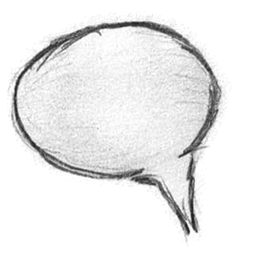
\includegraphics[width=0.4\linewidth]{Images/comment}
\end{center}
\end{frame}

\section{¿12 factores?}
\begin{frame}{12 factores}
\begin{itemize}
\item Metodología
\item Mejores prácticas
\item Manifesto 
\item https://12factor.net/
\end{itemize}
\end{frame}

\begin{frame}{12 factores cloud native (Heroku)}

\begin{columns}[T] % contents are top vertically aligned
	
	\begin{column}[T]{4cm} % alternative top-align that's better for graphics
		\begin{alertblock}{Frameworks}
			\begin{itemize}
				\item Config
				\item Backing service
				\item Disposability
			\end{itemize}
		\end{alertblock}
	\end{column}
	\begin{column}[T]{6cm} % each column can also be its own environment
		\begin{block}{Cloud}
			\begin{itemize}
				\item Codebase (Git-Flow)
				\item Dependencies (Maven)
				\item Build, Release, Run
				\item Processes
				\item Port binding
				\item Concurrency (Docker - k8s)
				\item Dev / Prod parity
				\item Logs
				\item Admin process
			\end{itemize}
		\end{block}
	\end{column}
\end{columns}

\end{frame}

\begin{frame}{Codebase}
\begin{itemize}
	\item Una base de código con múltiples entornos de despliegue
	\item Un repositorio por aplicación / microservicio
\end{itemize}

\begin{figure}
	\centering
	
\includegraphics[width=0.5\linewidth]{Images/121}
\end{figure}
\end{frame}


\begin{frame}{Dependencias}
\begin{itemize}
	\item Una aplicación cloud native no "depende" de algo en su entorno
	\item Dependencias isoladas y compilaciones repetibles
\end{itemize}

\begin{figure}
	\centering
	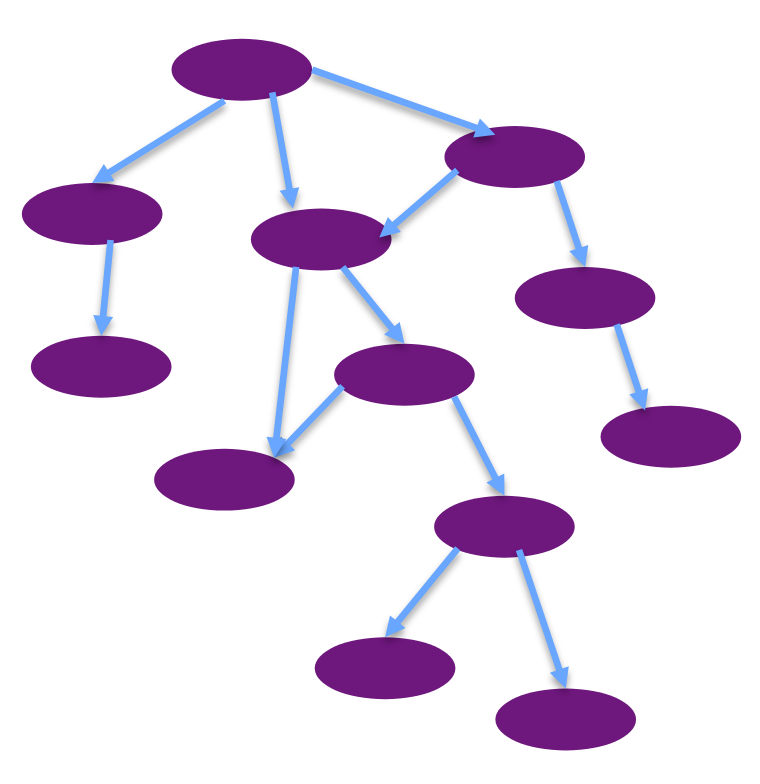
\includegraphics[width=0.5\linewidth]{Images/maven}
\end{figure}
\end{frame}


\begin{frame}{Configuración}
\begin{itemize}
	\item La configuración de una aplicación debe ser dinámica sin re-compilación/re-empaque 
	\item Configuraciones inyectables
\end{itemize}
\end{frame}


\begin{frame}{Backing services}
\begin{itemize}
	\item Acoplamiento debil. Siempre tratar backing services como componentes intercambiables y/o adjuntos
\end{itemize}

\begin{figure}
	\centering
	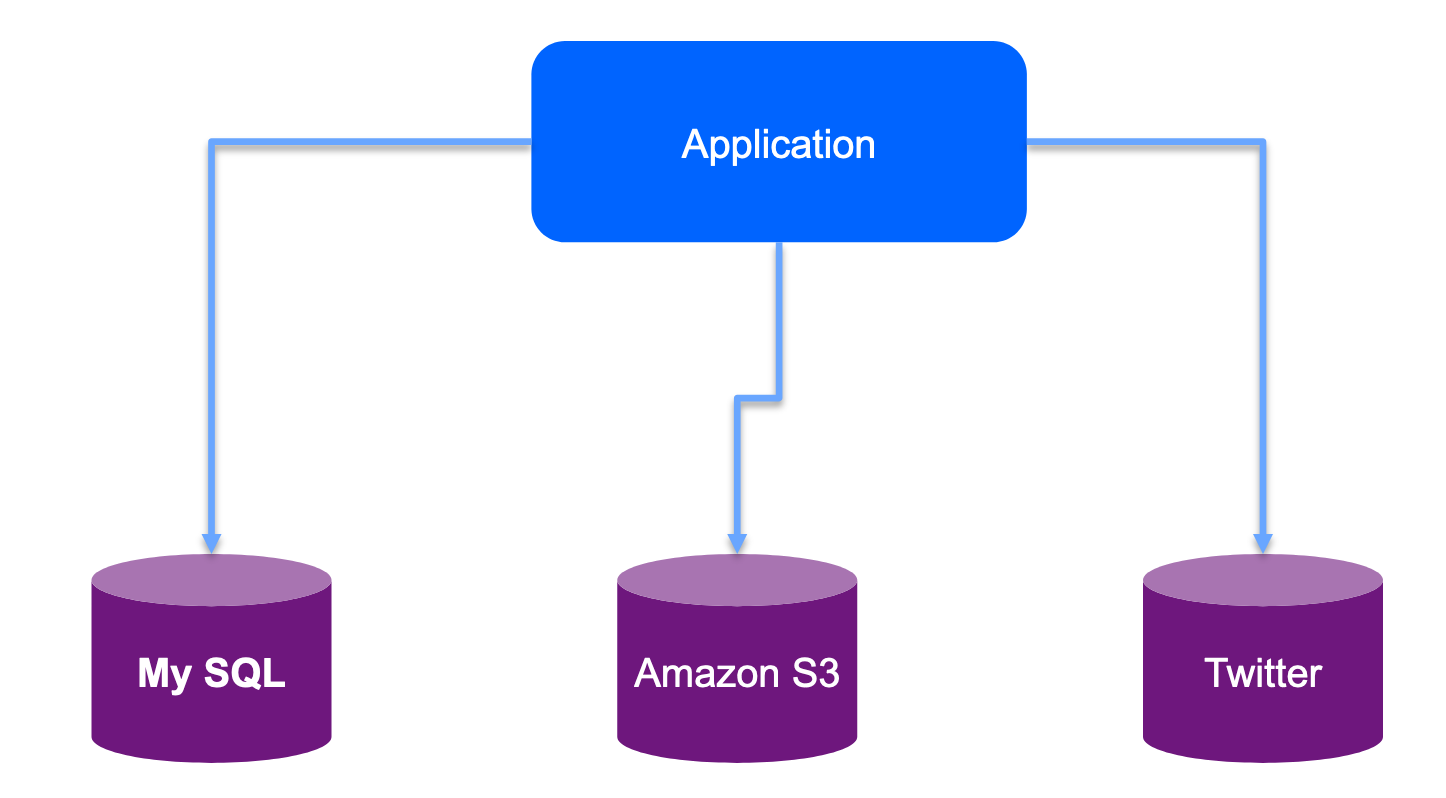
\includegraphics[width=0.5\linewidth]{Images/backing}
\end{figure}
\end{frame}

\begin{frame}{Build, release, run}
\begin{itemize}
	\item Separación de etapas de construcción, ejecución y lanzamiento
	\item CI/CD se hace obligatorio
\end{itemize}
\end{frame}

\begin{frame}{Procesos}
\begin{itemize}
	\item Ejecutar la aplicación como uno o más procesos sin estado
	\item REST, Stateless, sesiones portables con JWT
\end{itemize}
\begin{figure}
	\centering
	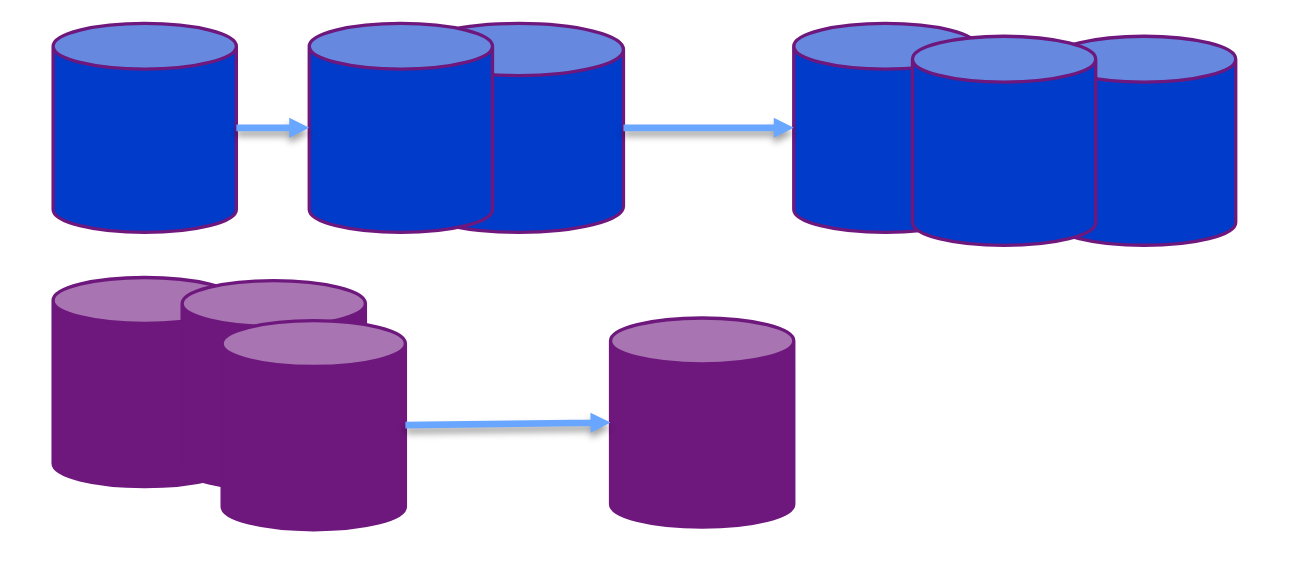
\includegraphics[width=0.5\linewidth]{Images/services}
\end{figure}
\end{frame}


\begin{frame}{Port binding}
\begin{itemize}
	\item Exponer los servicios con puertos dinámicos
	\item Kubernetes, Docker, etc.
\end{itemize}
\end{frame}

\begin{frame}{Concurrencia}
\begin{itemize}
	\item Aplicaciones escalan de forma independiente replicándose
	\item Las nubes escalan mediante copias independientes, sin estado
\end{itemize}
\end{frame}

\begin{frame}{Disposability}
\begin{itemize}
	\item Procesos arrancar rápido, mueren rápido, reinician rápido
	\item Procesos son tolerantes a fallas
\end{itemize}

\begin{figure}
	\centering
	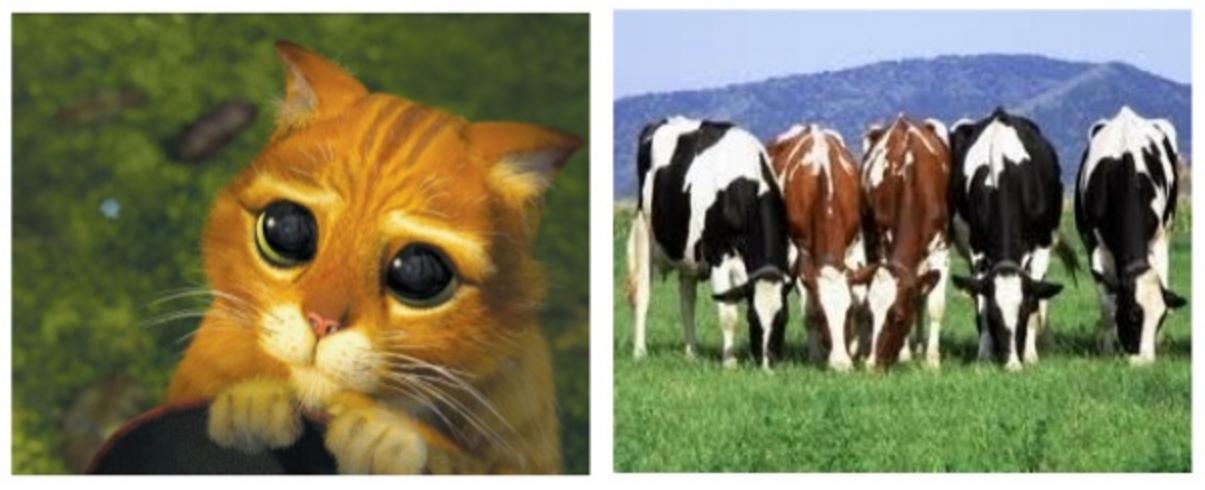
\includegraphics[width=0.5\linewidth]{Images/petvscattle}
\end{figure}
\end{frame}

\begin{frame}{Dev/Prod parity}
\begin{itemize}
	\item Entornos de desarrollo, certificación, producción lo más homogéneos posible
\end{itemize}
\end{frame}

\begin{frame}{Logs}
\begin{itemize}
	\item Manipular logs de n copias de n servicios (streams de eventos)
	\item Permitir el análisis posterior
\end{itemize}
\end{frame}

\begin{frame}{Admin process}
\begin{itemize}
	\item Manipular logs de n copias de n servicios (streams de eventos)
	\item Permitir el análisis posterior
\end{itemize}
\end{frame}


\begin{frame}{12 factores cloud native (Heroku)}

\begin{columns}[T] % contents are top vertically aligned
	
	\begin{column}[T]{4cm} % alternative top-align that's better for graphics
		\begin{alertblock}{Frameworks}
			\begin{itemize}
				\item Config
				\item Backing service
				\item Disposability
			\end{itemize}
		\end{alertblock}
	\end{column}
	\begin{column}[T]{6cm} % each column can also be its own environment
		\begin{block}{Cloud}
			\begin{itemize}
				\item Codebase (Git-Flow)
				\item Dependencies (Maven)
				\item Build, Release, Run
				\item Processes
				\item Port binding
				\item Concurrency (Docker - k8s)
				\item Dev / Prod parity
				\item Logs
				\item Admin process
			\end{itemize}
		\end{block}
	\end{column}
\end{columns}

\end{frame}


\begin{frame}{Monolito - Escalabilidad}
\begin{figure}
	\centering
	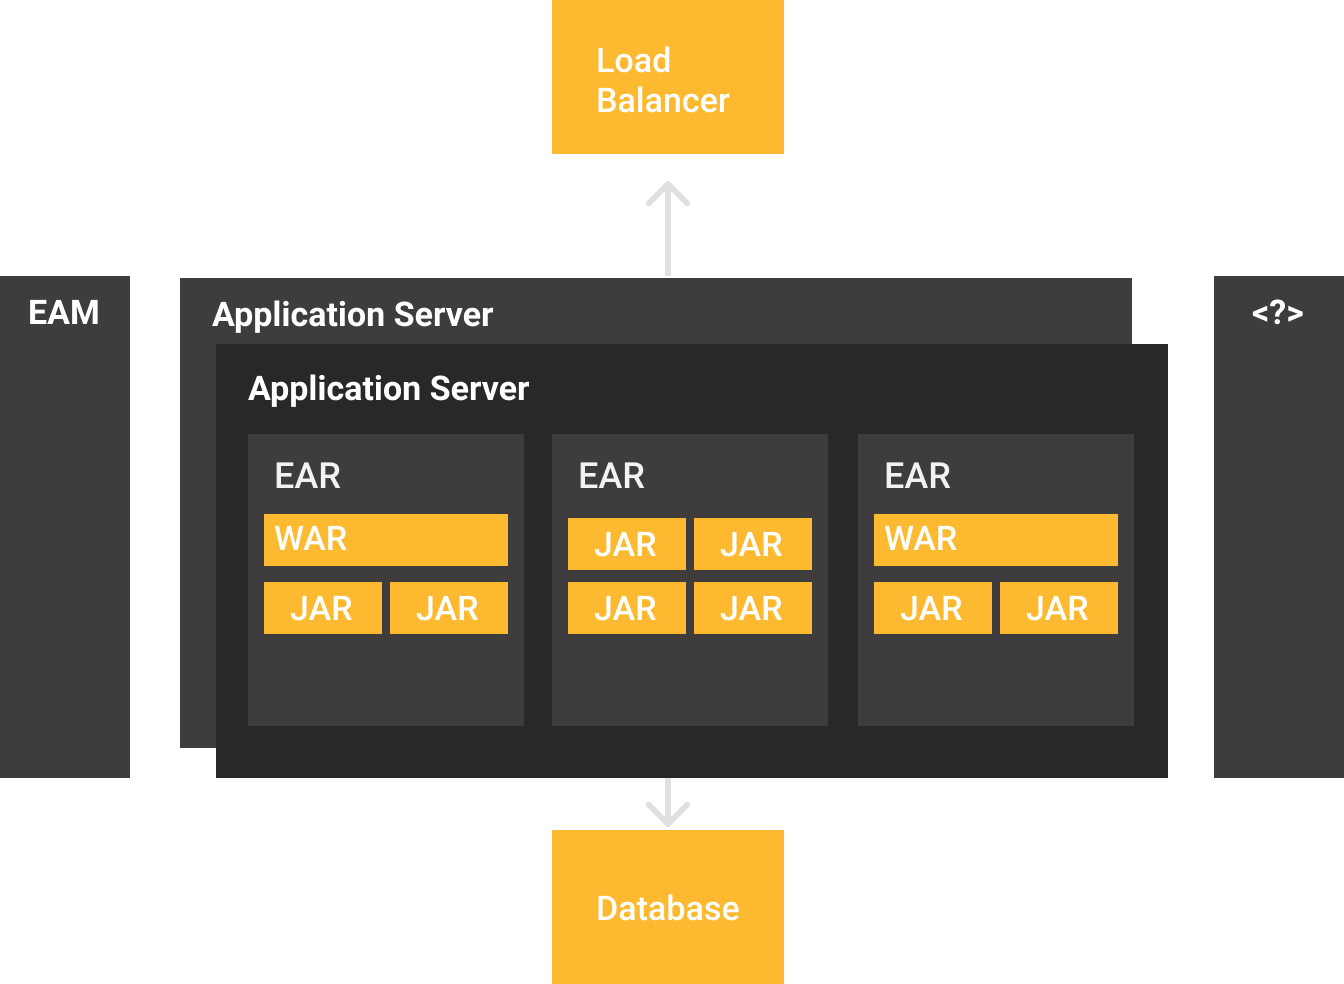
\includegraphics[width=0.7\linewidth]{Images/monolitos}
	\caption{Monólito}
\end{figure}
\end{frame}


\begin{frame}{Microservicios}
\begin{figure}
\centering
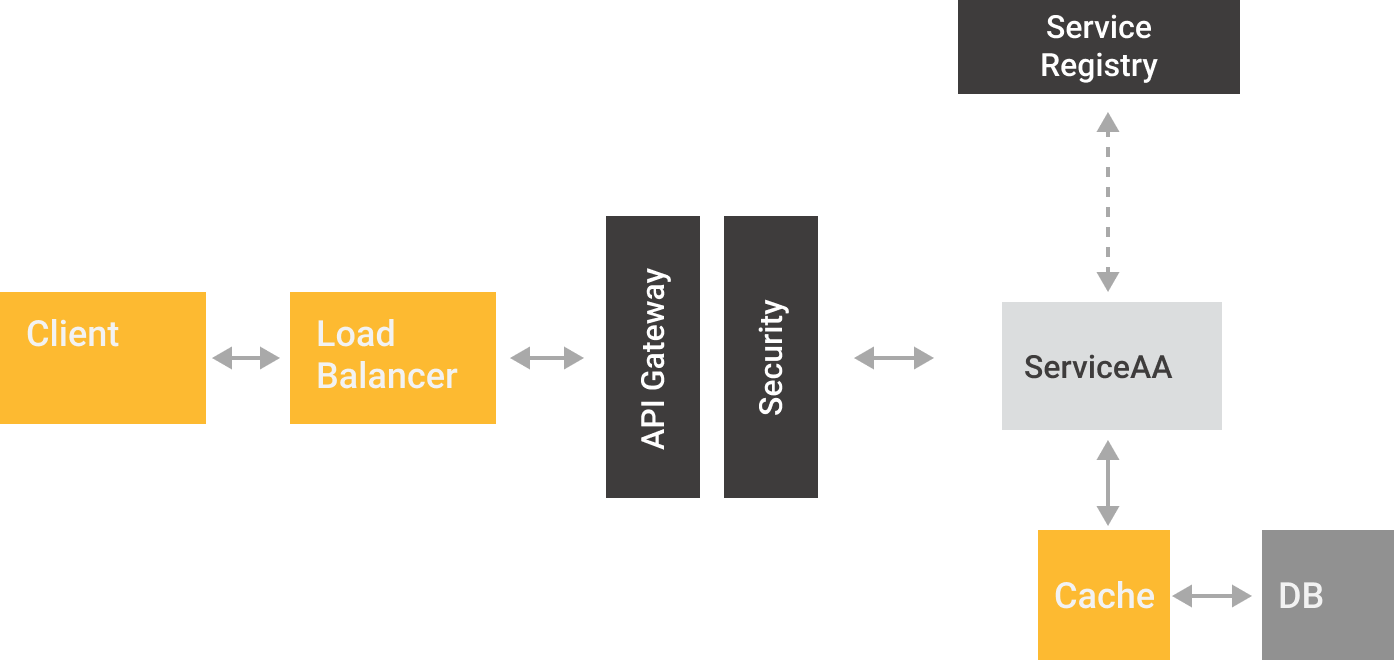
\includegraphics[width=\linewidth]{Images/microservicios}
\caption{Microservicios}
\end{figure}
\end{frame}


\section{Eclipse MicroProfile}

\begin{frame}{Eclipse MicroProfile}
\begin{figure}
	\centering
	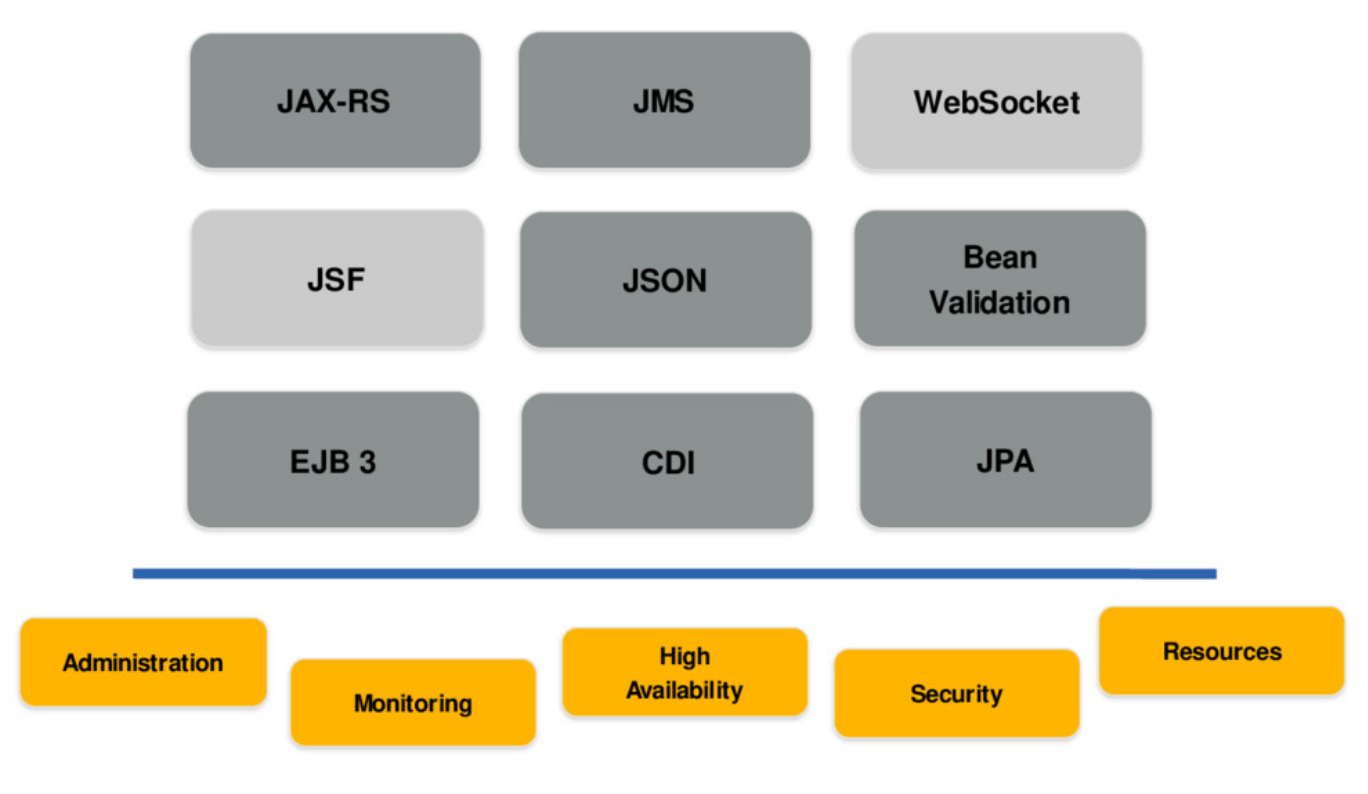
\includegraphics[width=\linewidth]{Images/javaeemicropancake}
	\caption{Credito: Reza Rahman}
\end{figure}
\end{frame}

\begin{frame}{Eclipse MicroProfile}
	\begin{figure}
		\centering
		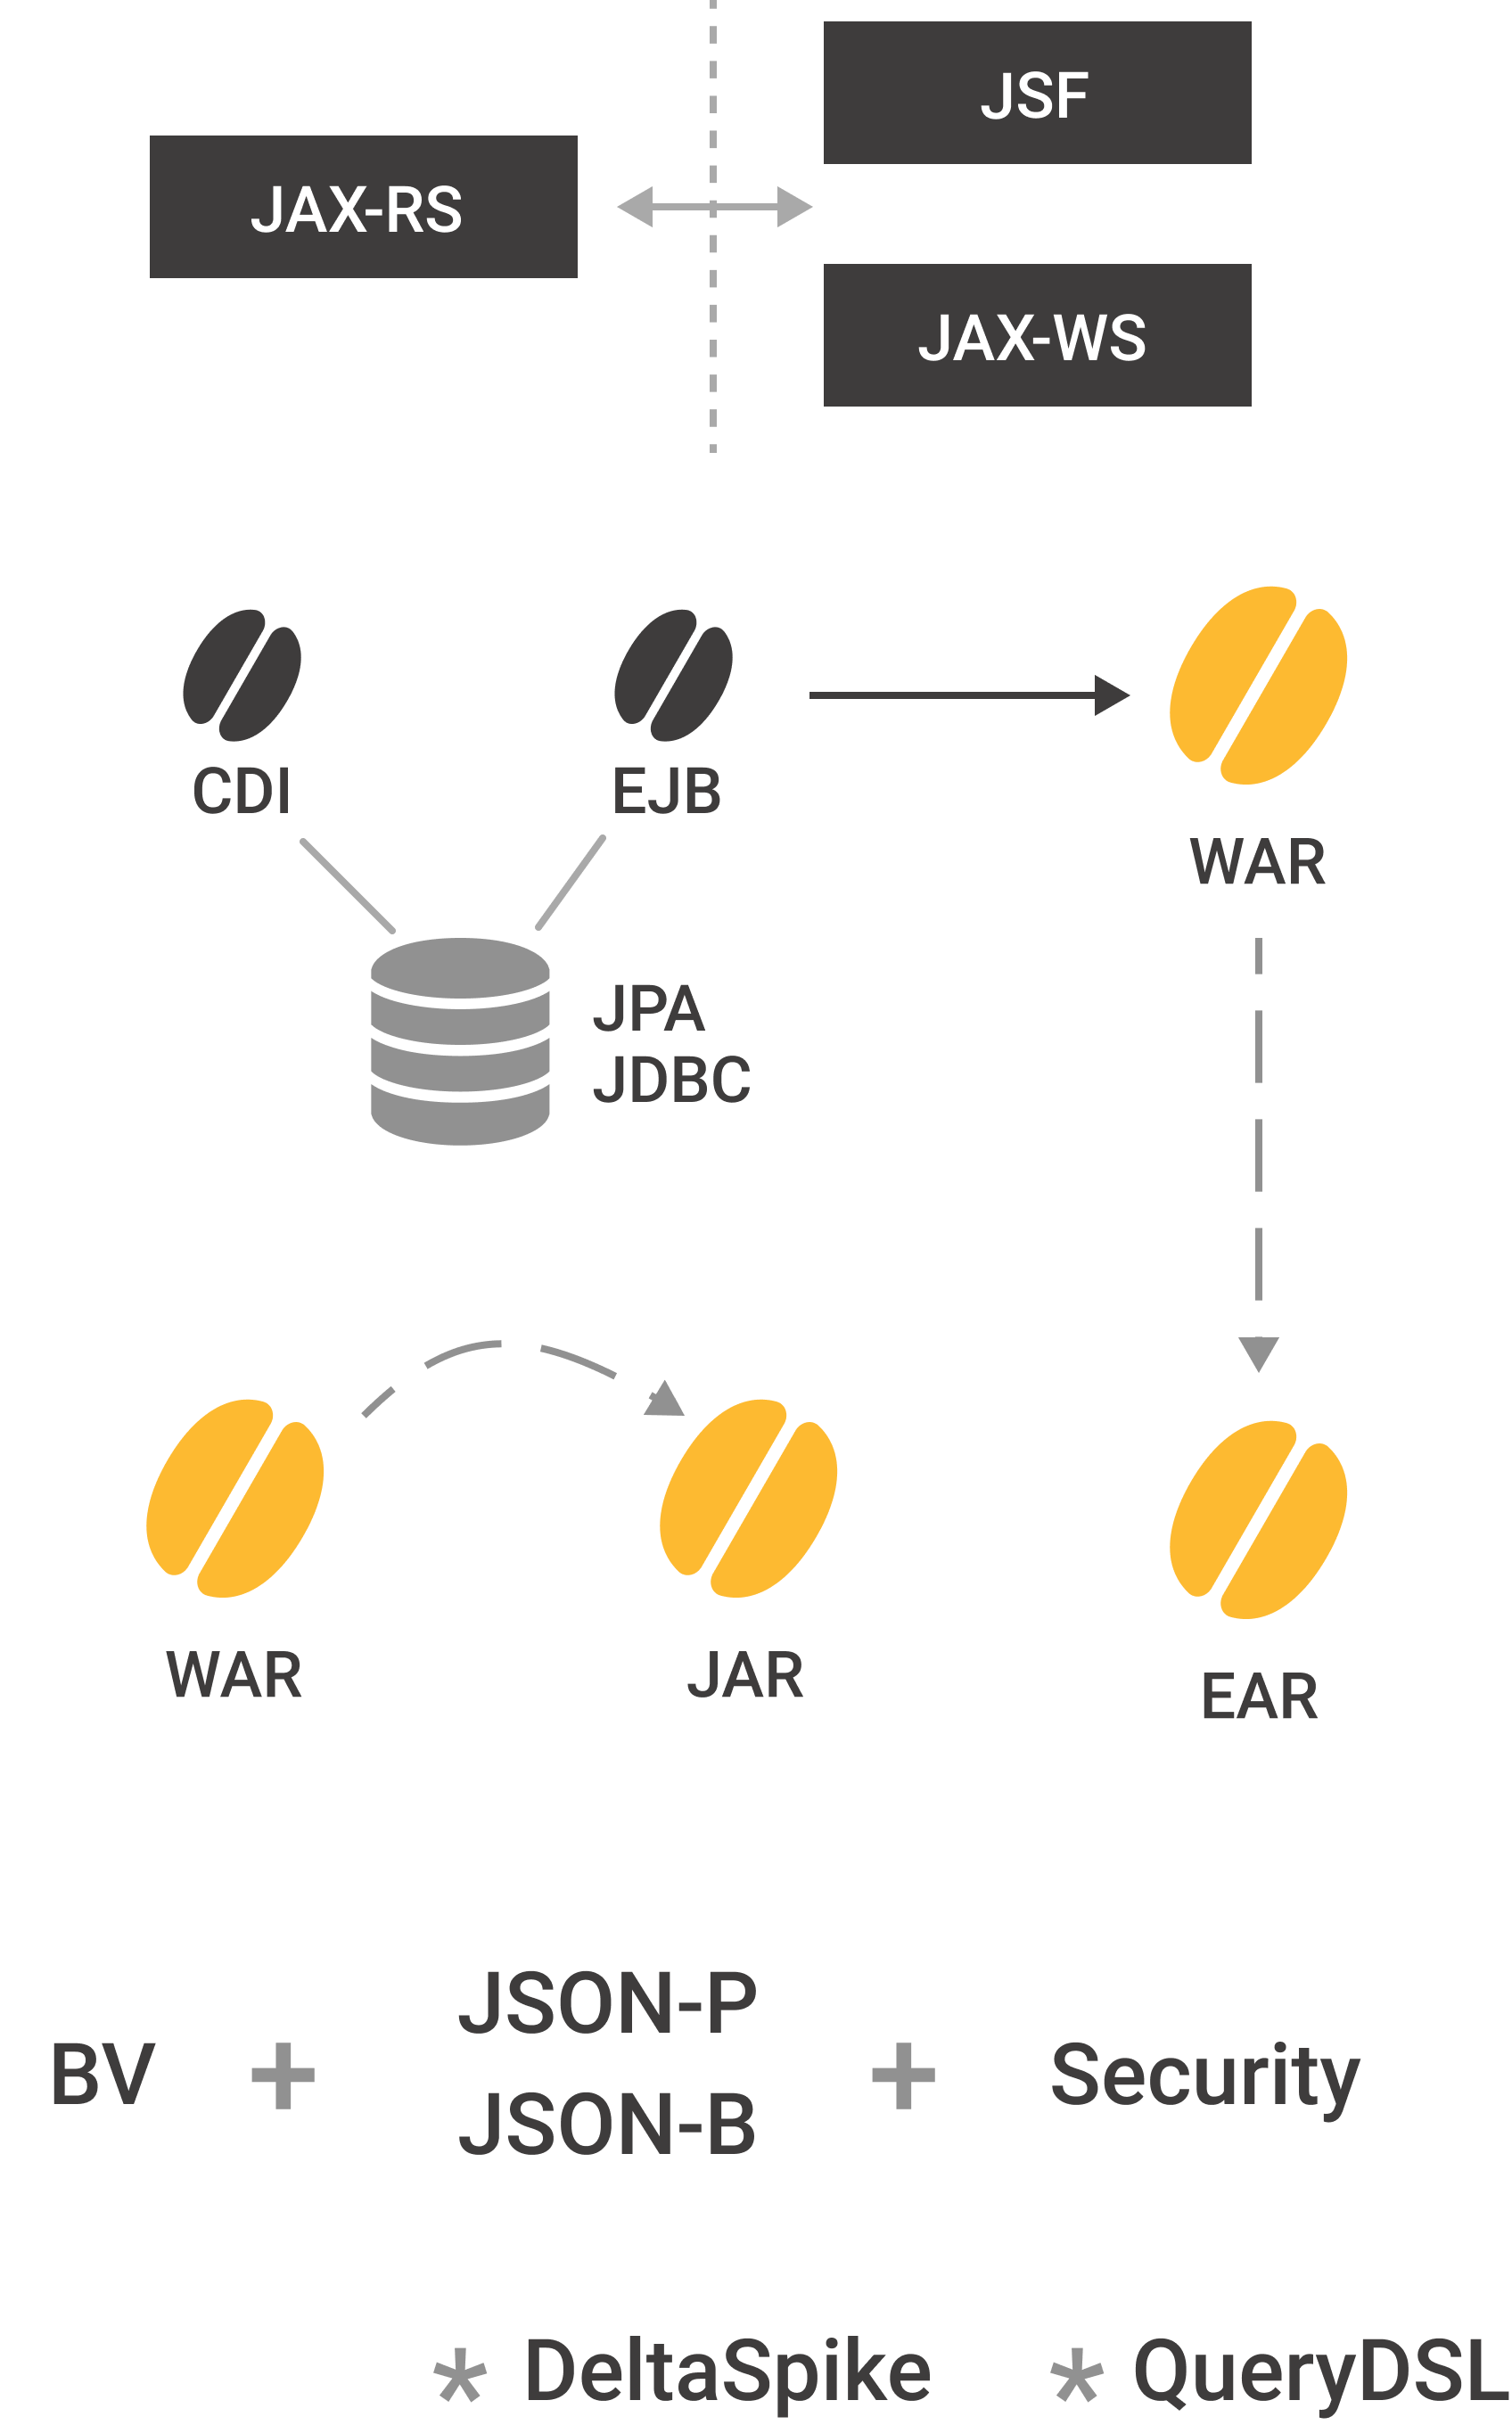
\includegraphics[width=0.5\linewidth]{Images/oldsetup}
	\end{figure}
\end{frame}

\begin{frame}{Eclipse MicroProfile}
\begin{figure}
	\centering
	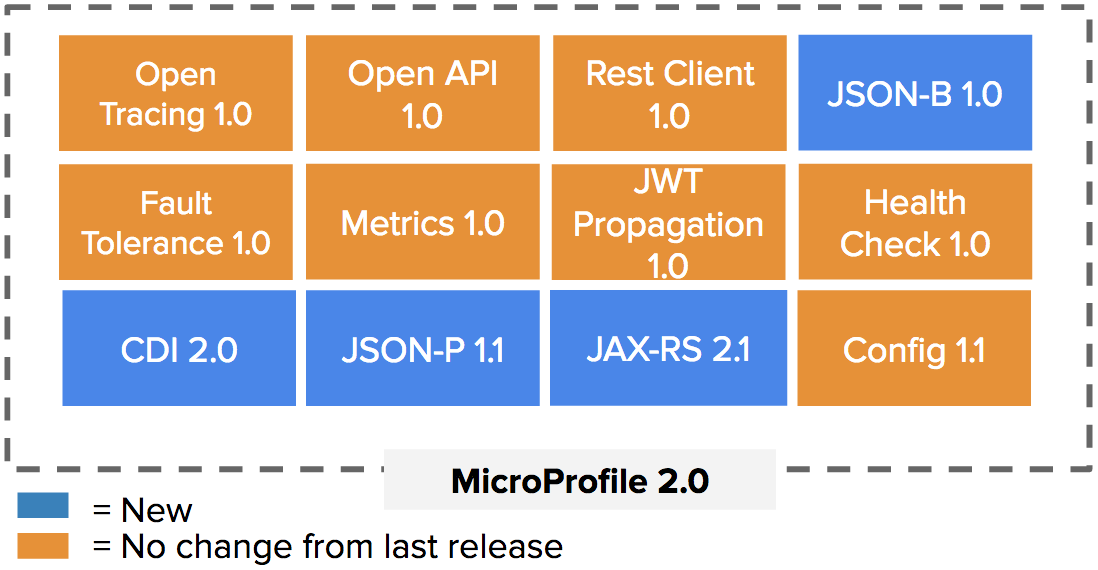
\includegraphics[width=\linewidth]{Images/mp5}
\end{figure}
\end{frame}

%TODO 12 fatores

\begin{frame}{Eclipse MicroProfile - Implementaciones}

Bibliotecas
\begin{itemize}
	\item SmallRye (Red Hat)
	\item Hammock
	\item Apache Geronimo
	\item Fujitsu Launcher
\end{itemize}
	
JEAS - Fat Jar
\begin{itemize}
	\item Dropwizard
	\item KumuluzEE
	\item Helidon (Oracle)
	\item Open Liberty (IBM)
	\item Apache Meecrowave
	\item Thorntail (Red Hat)
	\item Quarkus (Red Hat)
\end{itemize}

https://wiki.eclipse.org/MicroProfile/Implementation

\end{frame}
\begin{frame}{Eclipse MicroProfile - Implementaciones}

Micro server
\begin{itemize}
	\item Payara Micro
	\item TomEE JAX-RS
\end{itemize}

Full server
\begin{itemize}
	\item Payara Application Server
	\item JBoss Application Server / Wildfly Application Server
	\item WebSphere Liberty (IBM)
\end{itemize}

https://wiki.eclipse.org/MicroProfile/Implementation
\end{frame}

\begin{frame}[fragile]{Eclipse MicroProfile on Payara 5}
\begin{lstlisting}
<dependency>
	<groupId>org.eclipse.microprofile</groupId>
	<artifactId>microprofile</artifactId>
	<type>pom</type>
	<version>2.0.1</version>
	<scope>provided</scope>
</dependency>
\end{lstlisting}
\end{frame}


\section{Demo}
\begin{frame}{Kotlin + Jakarta EE + MicroProfile  - Demo}

\begin{itemize}
	\item Kotlin 1.3
	\item Libraries - SLF4J, Flyway, PostgreSQL
	\item Jakarta EE 8 - EJB, JPA
	\item MicroProfile - CDI, JAX-RS, MicroProfile Config
	\item Testing - Arquillian, JUnit, Payara Embedded
\end{itemize}


\normalsize  \url{https://dzone.com/articles/the-state-of-kotlin-for-jakarta-eemicroprofile-tra}\\
\normalsize  \url{https://github.com/tuxtor/integrum-ee}
\end{frame}

\begin{frame}{Kotlin + Jakarta EE + MicroProfile  - Demo}
\begin{figure}
\centering
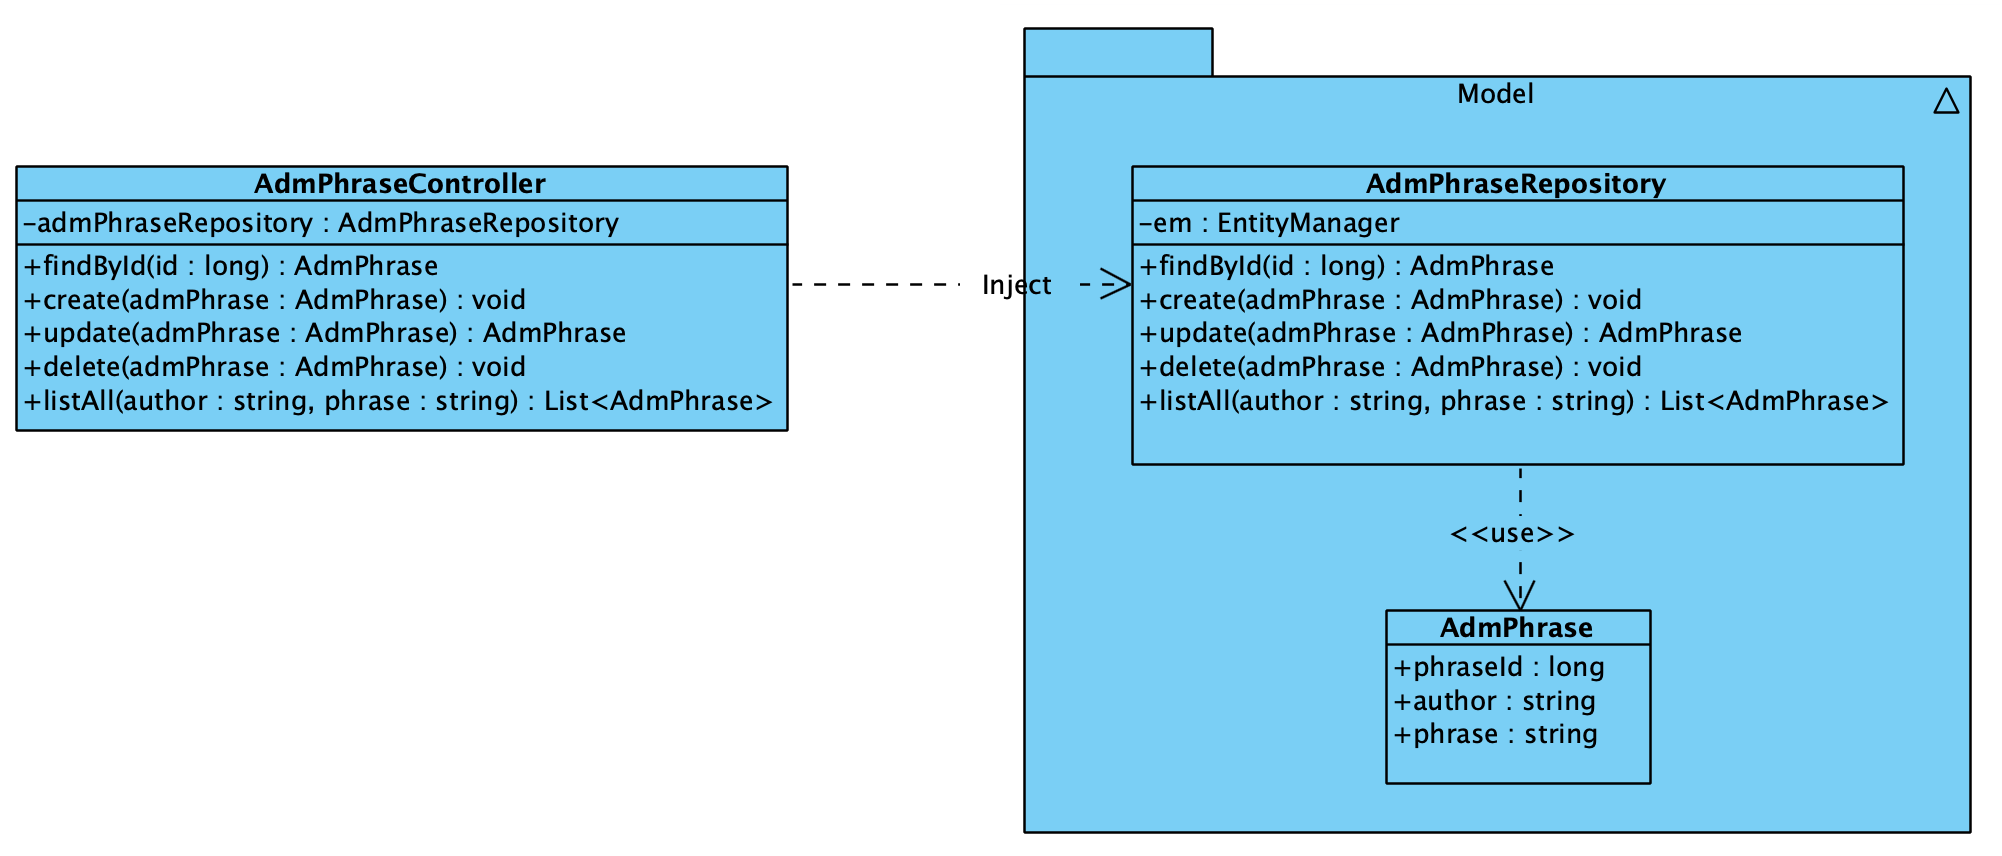
\includegraphics[width=\linewidth]{Images/integrum-ee}
\end{figure}
\end{frame}

\begin{frame}{Kotlin + Jakarta EE + MicroProfile  - Demo}
\begin{figure}
\centering
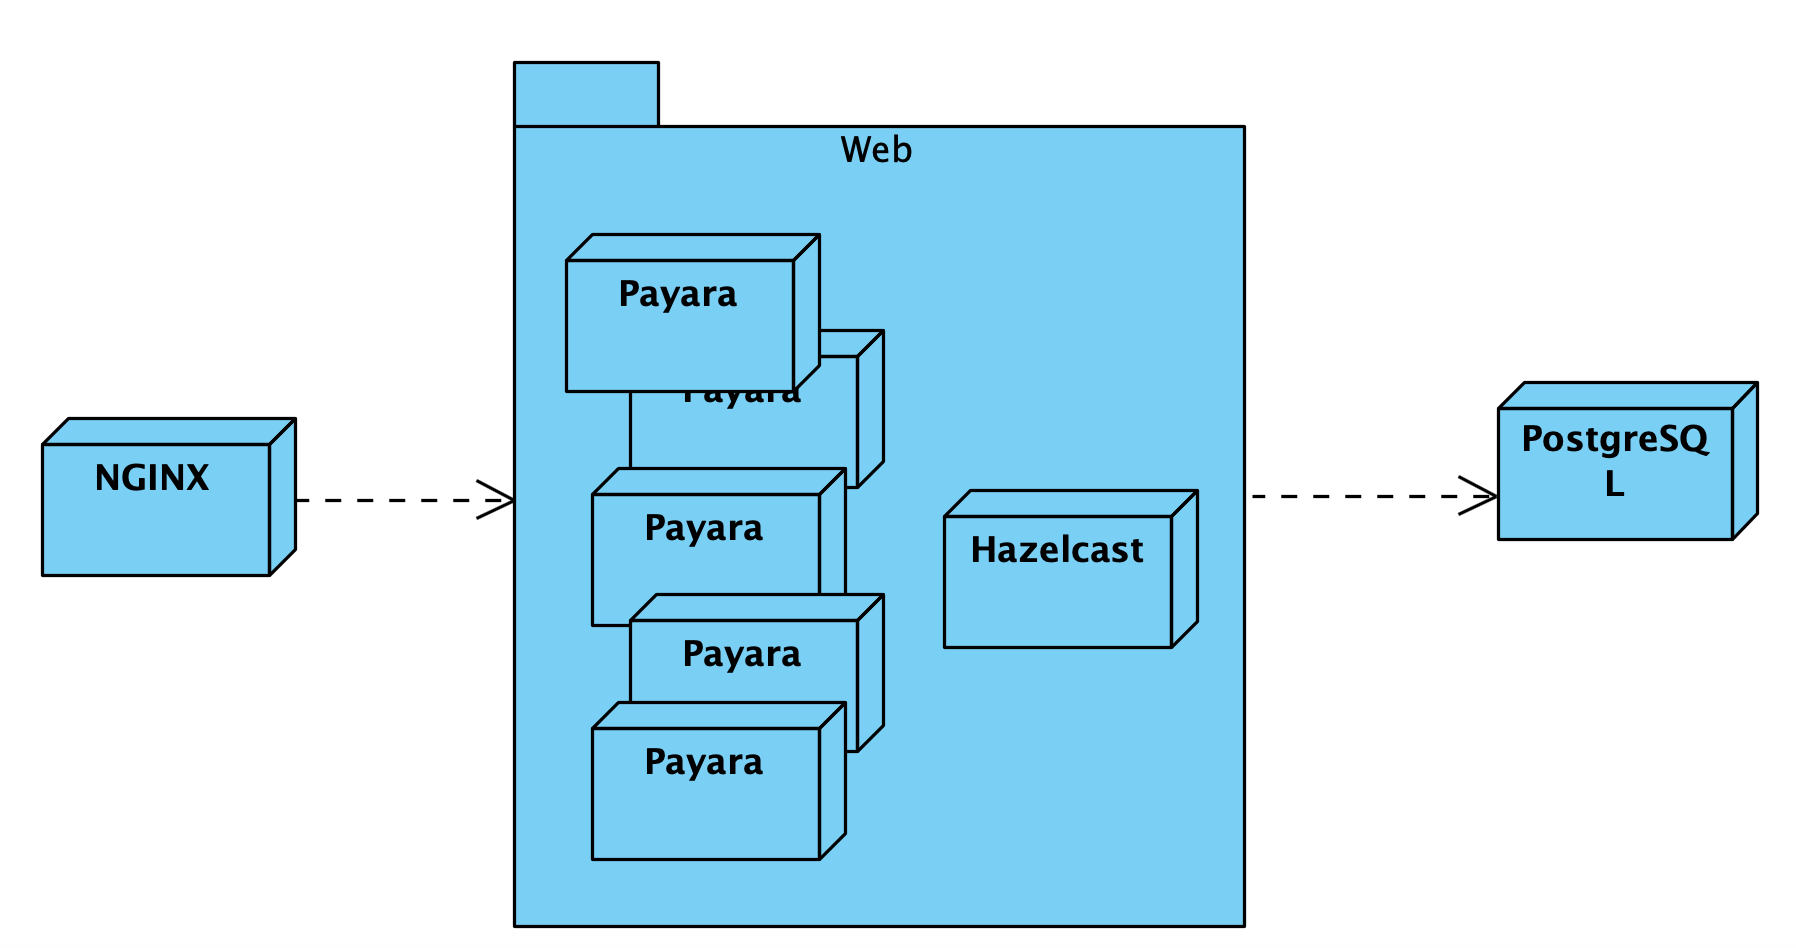
\includegraphics[width=\linewidth]{Images/integrum-deployment}
\end{figure}
\end{frame}



\begin{frame}{Oracle Cloud}
\begin{figure}
\centering
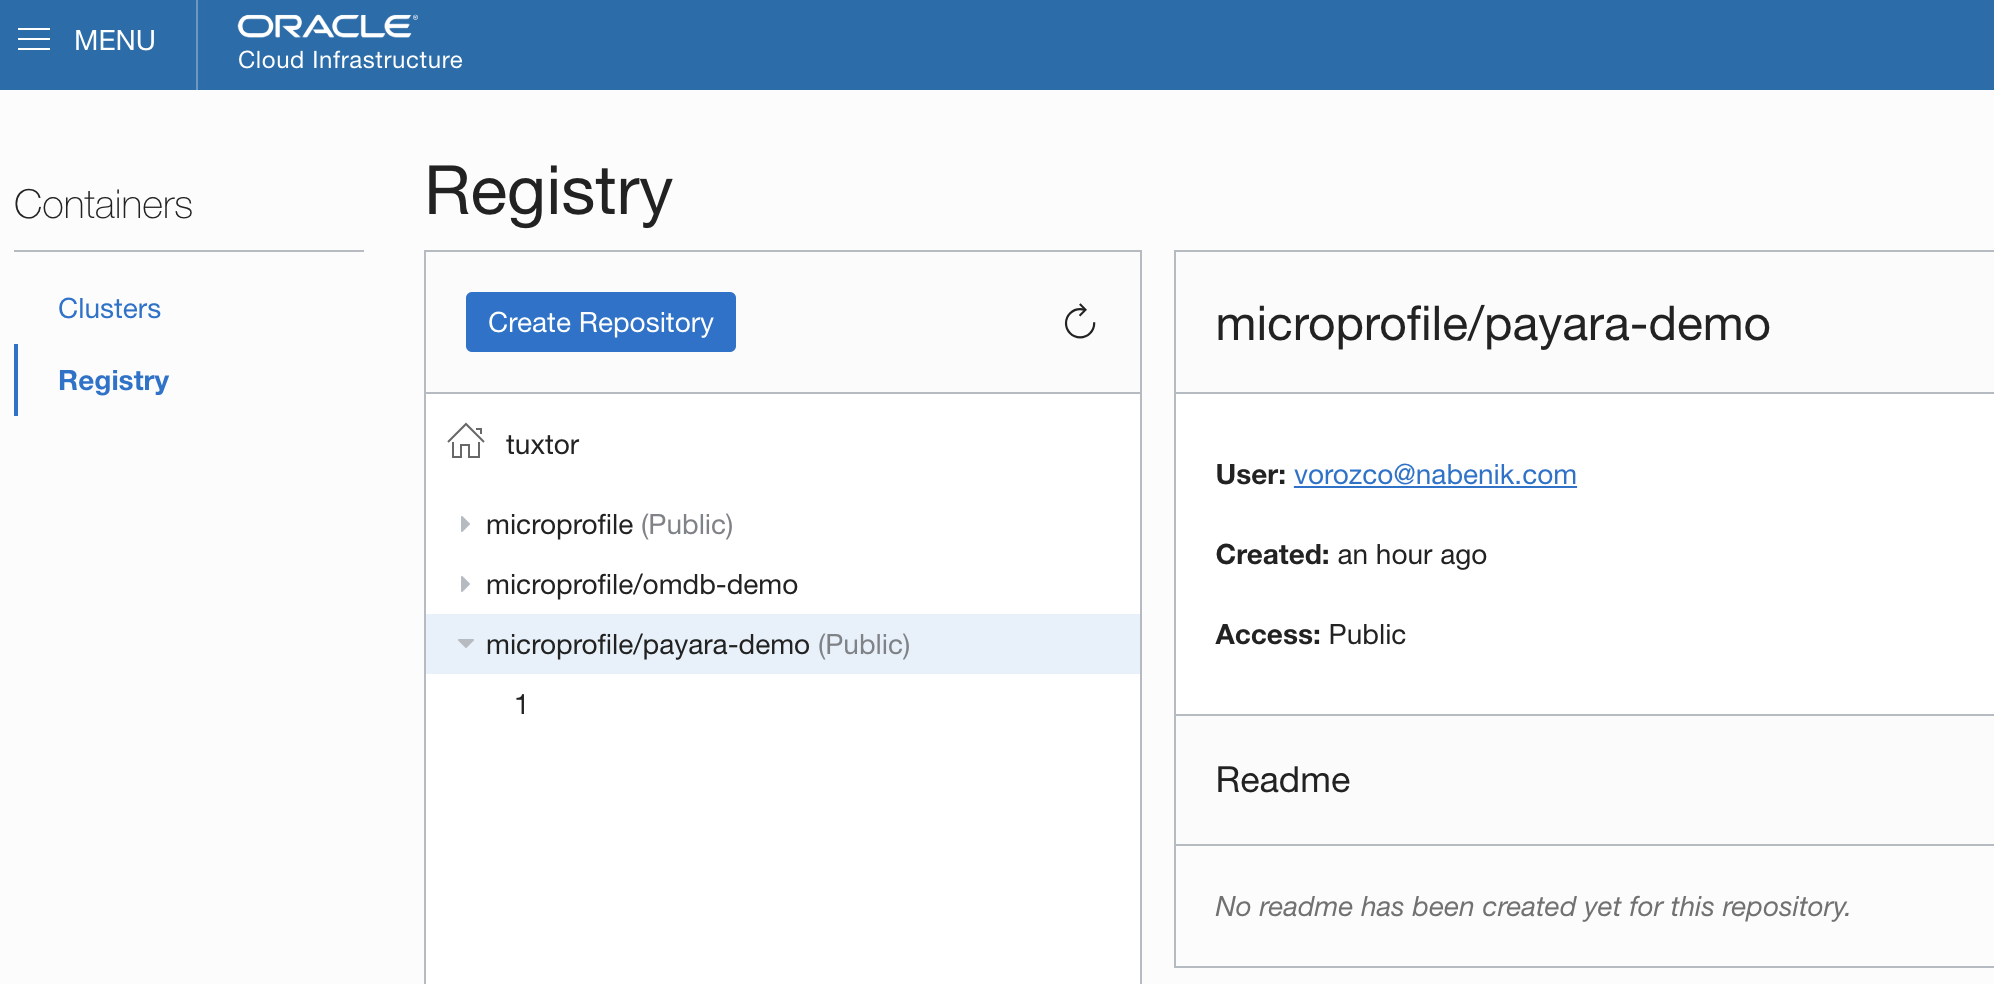
\includegraphics[width=0.95\linewidth]{Images/oc1}
\end{figure}
\end{frame}

\begin{frame}{Oracle Cloud}
\begin{figure}
\centering
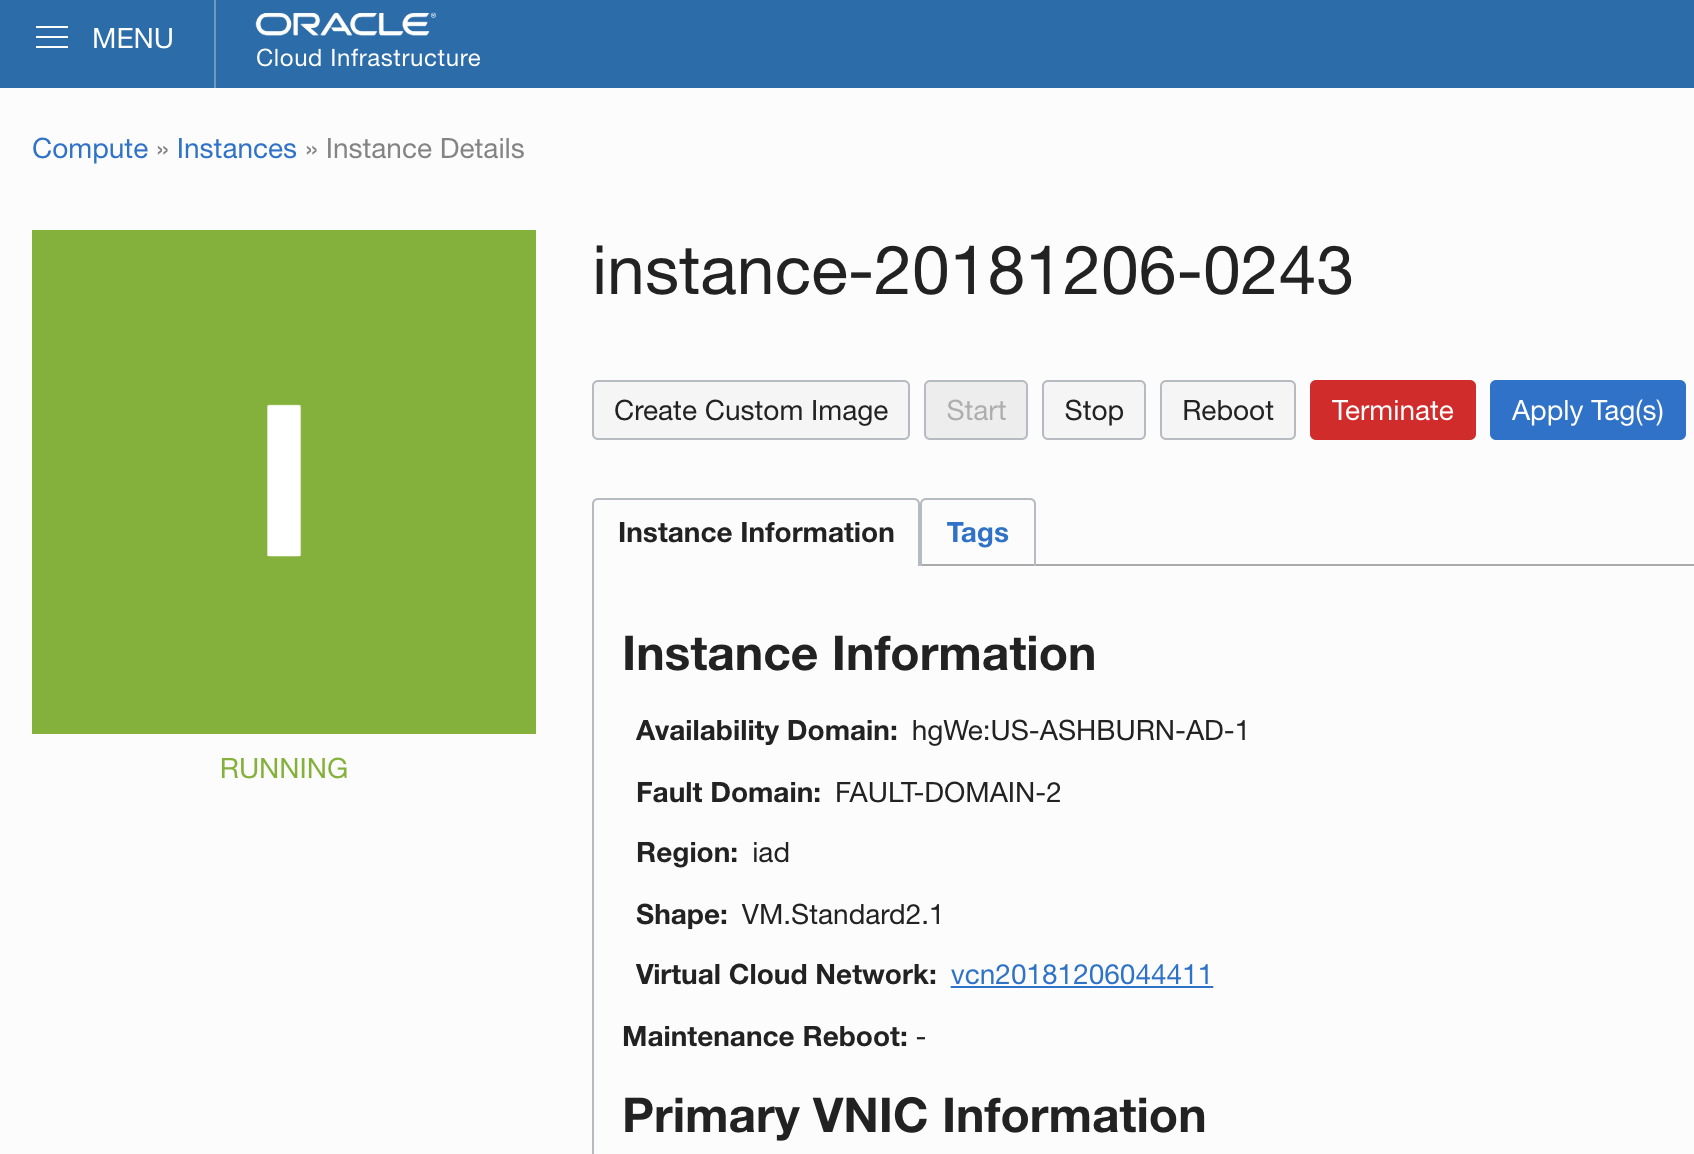
\includegraphics[width=0.95\linewidth]{Images/oc2}
\end{figure}
\end{frame}

\begin{frame}{Oracle Cloud}
\begin{figure}
\centering

\includegraphics[width=\linewidth]{Images/oc3}
\end{figure}

\begin{figure}
\centering
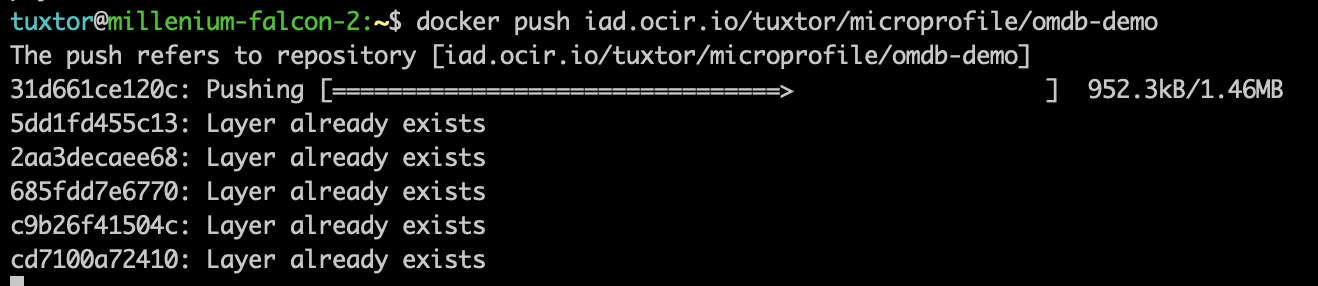
\includegraphics[width=\linewidth]{Images/oc4}
\end{figure}
\end{frame}

\begin{frame}{Oracle Cloud}

\begin{figure}
\centering
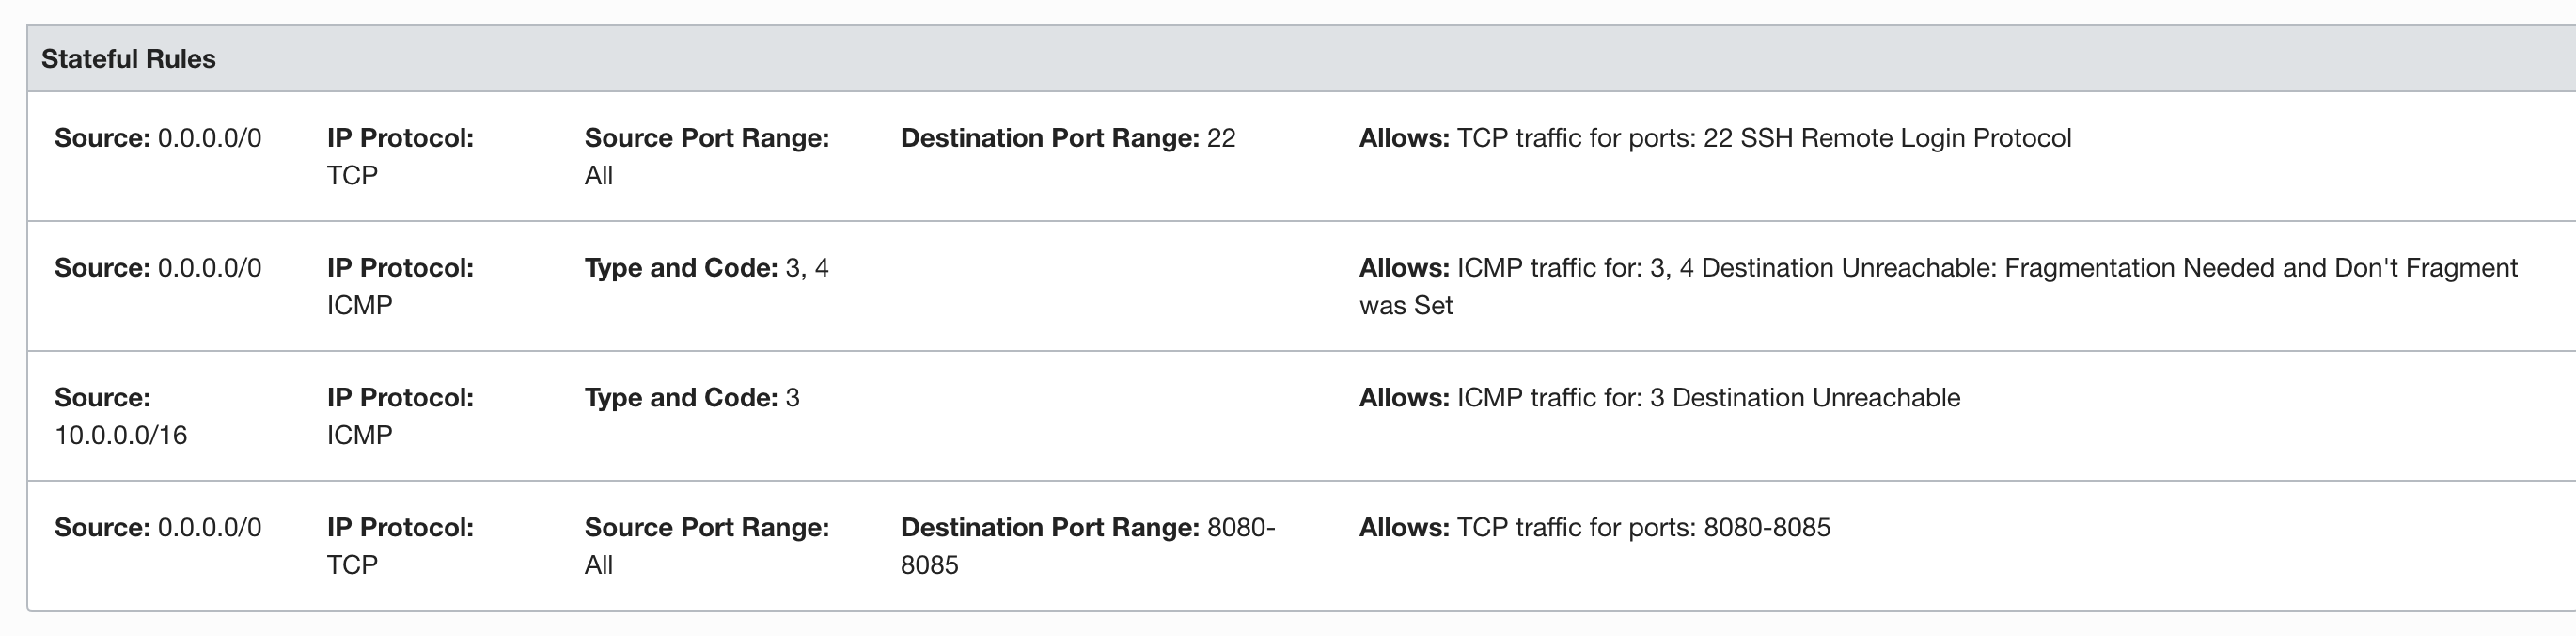
\includegraphics[width=\linewidth]{Images/oc5}
\end{figure}
\end{frame}

\begin{frame}{Config}
\begin{figure}
	\centering
	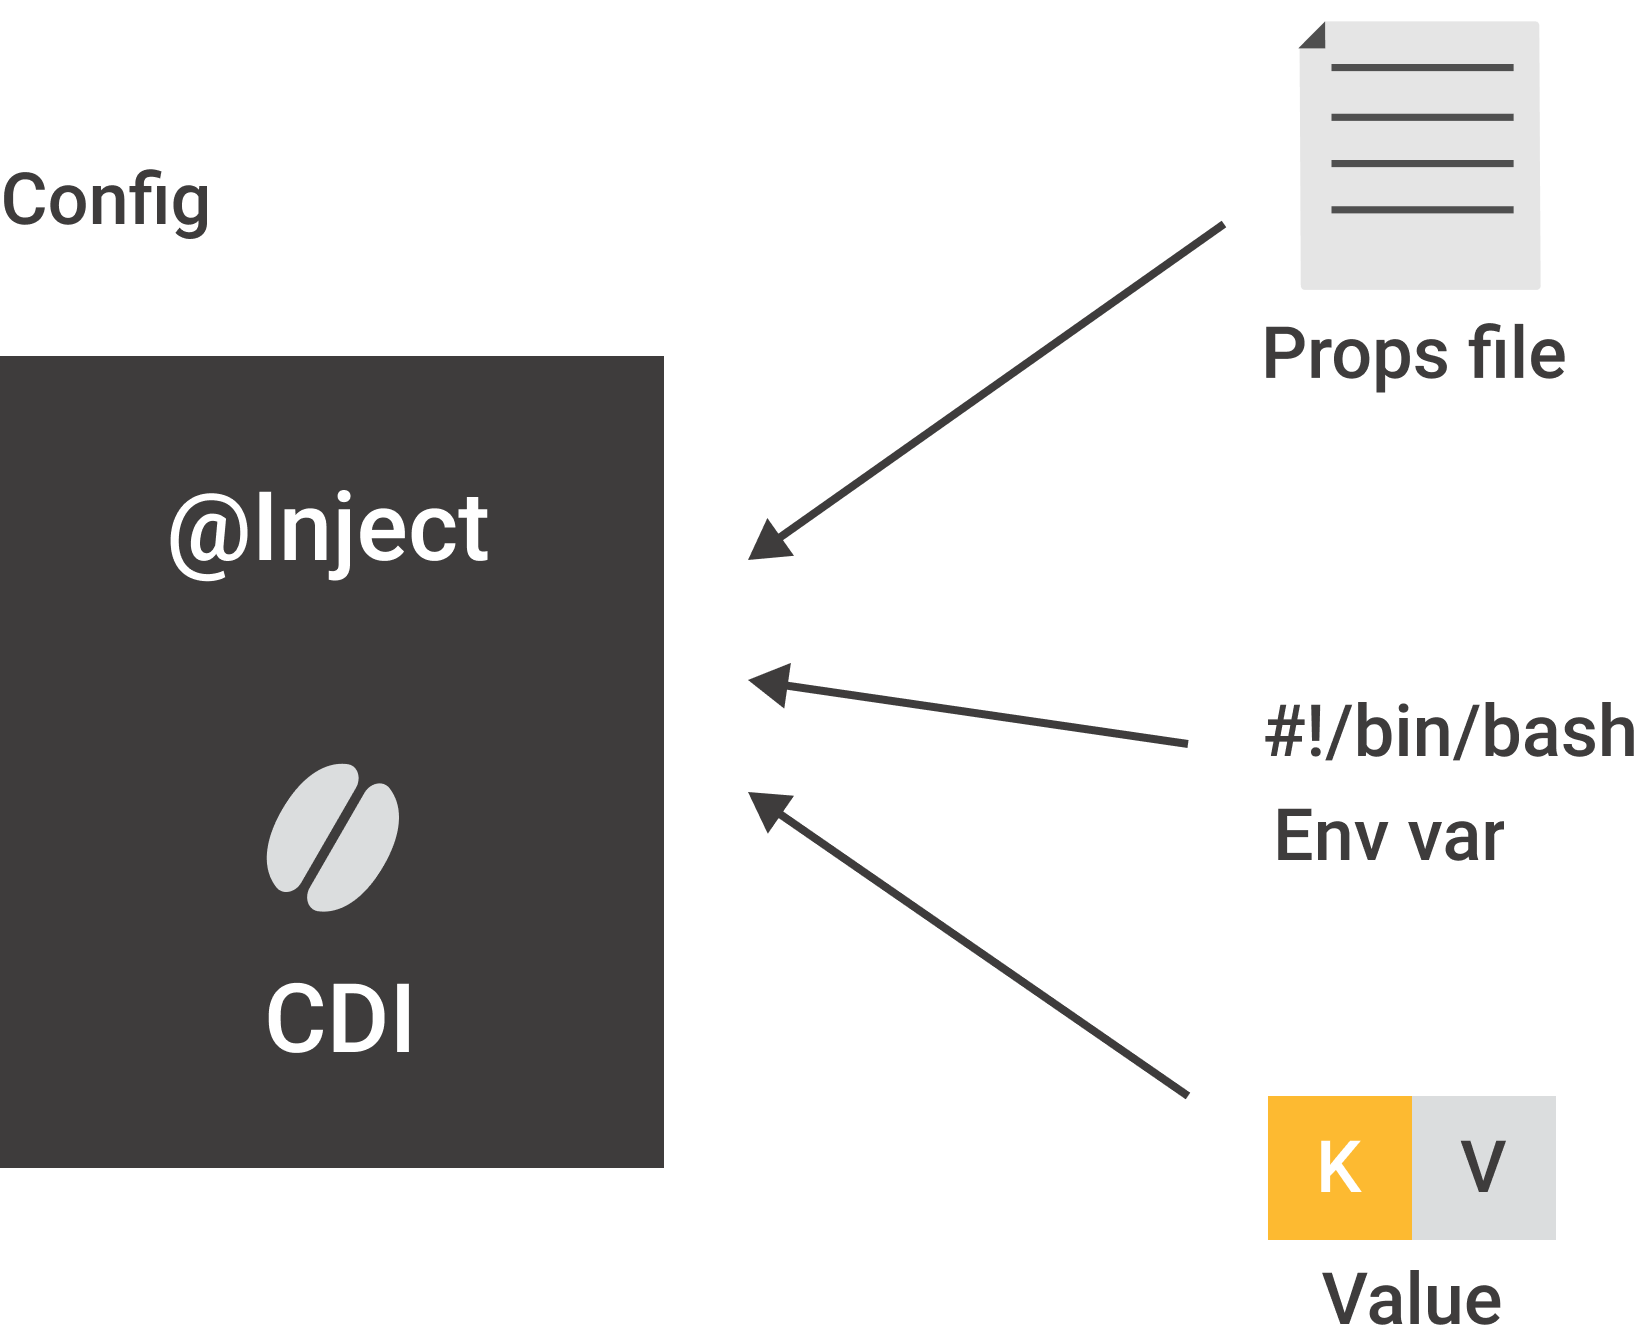
\includegraphics[width=0.75\linewidth]{Images/config}
\end{figure}
\end{frame}




\begin{frame}[fragile]{Config}
\begin{lstlisting}
@Inject
<@\textcolor{red}{@ConfigProperty(name = "omdbservice.url")}@>
String omdbDaemonServiceUrl;
\end{lstlisting}

Ext. de la configuración (VM, Docker, Kubernetes)
\end{frame}


\begin{frame}{Fault Tolerance}
\begin{figure}
	\centering
	
\includegraphics[width=0.75\linewidth]{Images/faulttolerance}
\end{figure}
\end{frame}

\begin{frame}{Metrics}
\begin{figure}
	\centering
	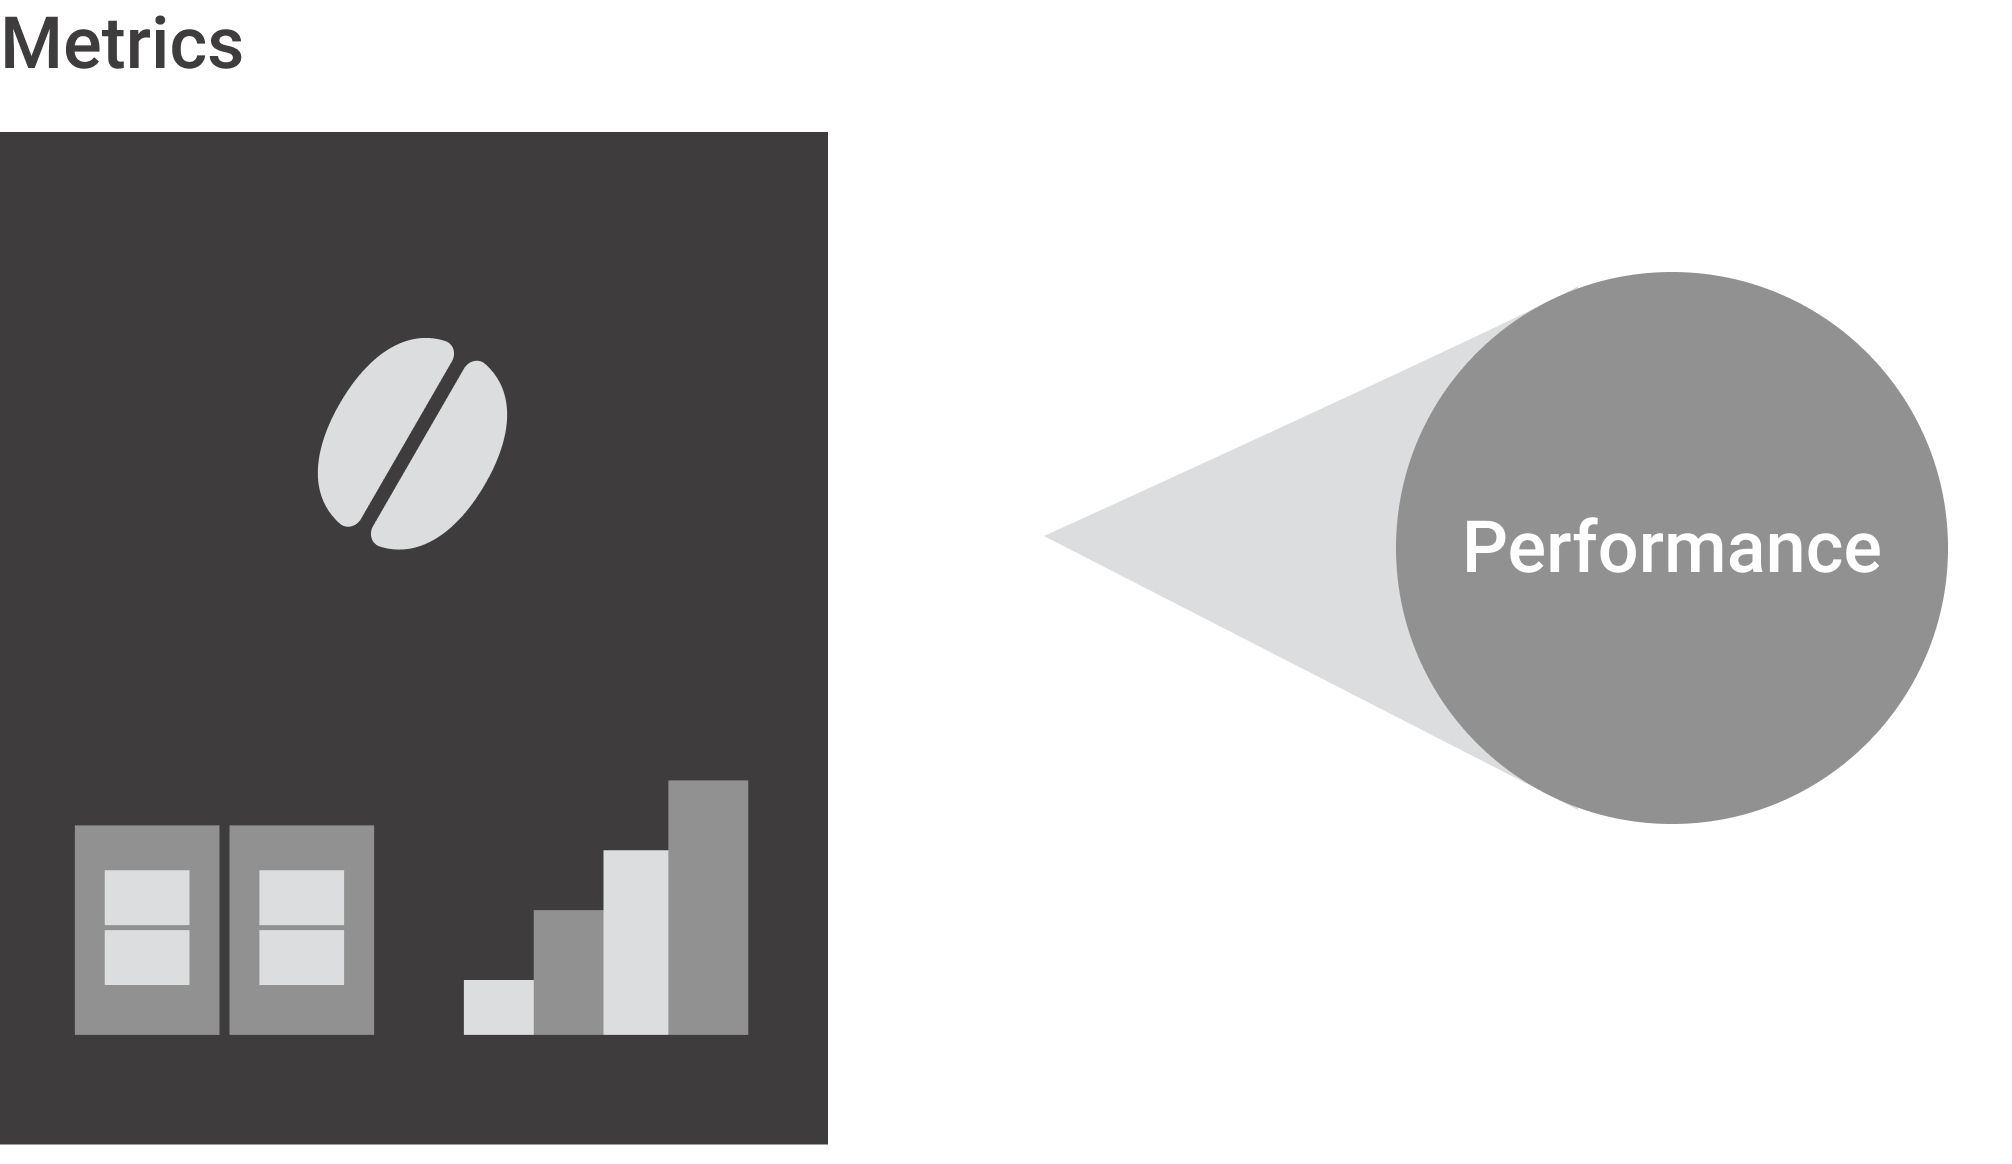
\includegraphics[width=0.75\linewidth]{Images/metrics}
\end{figure}
\end{frame}




\begin{frame}{Fault Tolerance + Metrics}

\begin{itemize}
	\item \textit{Fault Tolerance} depende de la existencia de metricas, las metricas se exponen  mediante \textit{Metrics}
\end{itemize}

\begin{figure}
	\centering
	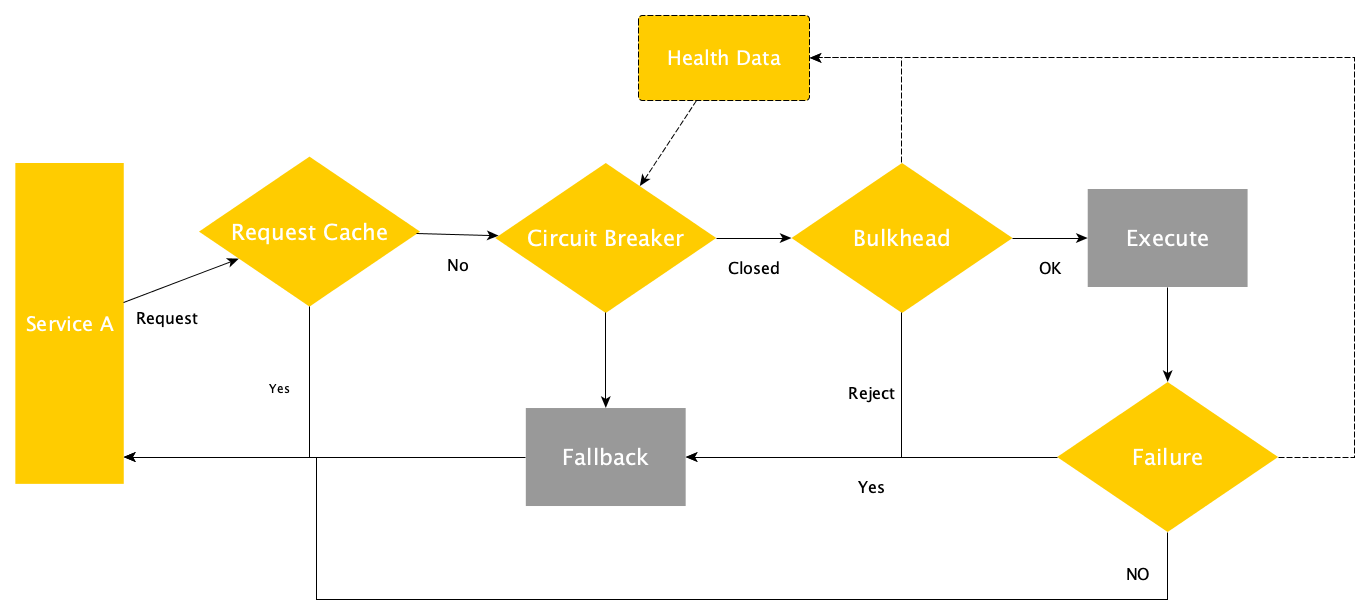
\includegraphics[width=\linewidth]{Images/falldata}
\end{figure}

\end{frame}


\begin{frame}{Fault tolerance}

Reglas de evaluación y alternativas
\begin{itemize}
\item Circuit Breaker
\item Bulkhead
\item Retry
\item Timeout
\item Fallback
\end{itemize}

\end{frame}


\begin{frame}[fragile]{Fault tolerance - Fallback, Timeout}
\begin{lstlisting}
@GET
@Path("/{id:[a-z]*[0-9][0-9]*}")
<@\textcolor{red}{@Fallback(fallbackMethod = "findByIdFallBack")}@>
<@\textcolor{red}{@Timeout(TIMEOUT)}@>
public Response findById(@PathParam("id") 
final String imdbId) {
...
}

public Response findByIdFallBack(@PathParam("id") 
final String imdbId) {
...
}
\end{lstlisting}
\end{frame}


\begin{frame}{Métricas}

\begin{itemize}
	\item JSON or OpenMetrics (Prometheus)
	\item Vendor
	\item Base
	\item Application
\end{itemize}

¿Cuales? 
\begin{itemize}
	\item Counted
	\item Gauge
	\item Metered
	\item Timed
	\item Histogram
\end{itemize}

\end{frame}

\begin{frame}[fragile]{Metrics - Counted}
\begin{lstlisting}
@Inject
<@\textcolor{red}{@Metric}@>
Counter failedQueries;
\end{lstlisting}

\begin{lstlisting}
@GET
@Path("/{id:[a-z]*[0-9][0-9]*}")
<@\textcolor{red}{@Fallback(fallbackMethod = "findByIdFallBack")}@>
<@\textcolor{red}{@Timeout(TIMEOUT)}@>
public Response findById(@PathParam("id") 
final String imdbId) {
...
}

public Response findByIdFallBack(@PathParam("id") 
final String imdbId) {
	...
	<@\textcolor{red}{failedQueries.inc();}@>
}
\end{lstlisting}
\end{frame}

\begin{frame}[fragile]{Metrics - Gauge}
Inc-dec en tiempo real
\begin{lstlisting}
<@\textcolor{red}{
@Gauge(unit = "ExternalDatabases",
	name = "movieDatabases", absolute = true)
}@>
public long getDatabases() {
	return 99; //Any value
}
\end{lstlisting}

\lstinline|/metrics/application/movieDatabases|
\end{frame}

%\begin{frame}[fragile]{Metrics - Metered}
%Events rate
%\begin{lstlisting}
%@Metered(name = "moviesRetrieved",
%	unit = MetricUnits.MINUTES,
%	description = "Metrics to monitor movies",
%	absolute = true)
%public Response findExpandedById(
%	@PathParam("id") final Long id) 
%\end{lstlisting}

%\lstinline|/metrics/application/movieDatabases|
%\end{frame}

%\begin{frame}[fragile]{Metrics- Timed}
%Desempeño y retraso
%\begin{lstlisting}
%@Timed(name = "moviesDelay",
%	description = "Time to retrieve a movie",
%	unit = MetricUnits.MINUTES,
%	absolute = true)
%public Response findExpandedById(
%	@PathParam("id") final Long id) 
%\end{lstlisting}

%\lstinline|/metrics/application/moviesDelay|
%\end{frame}


\begin{frame}{Health Check}
\begin{figure}
	\centering
	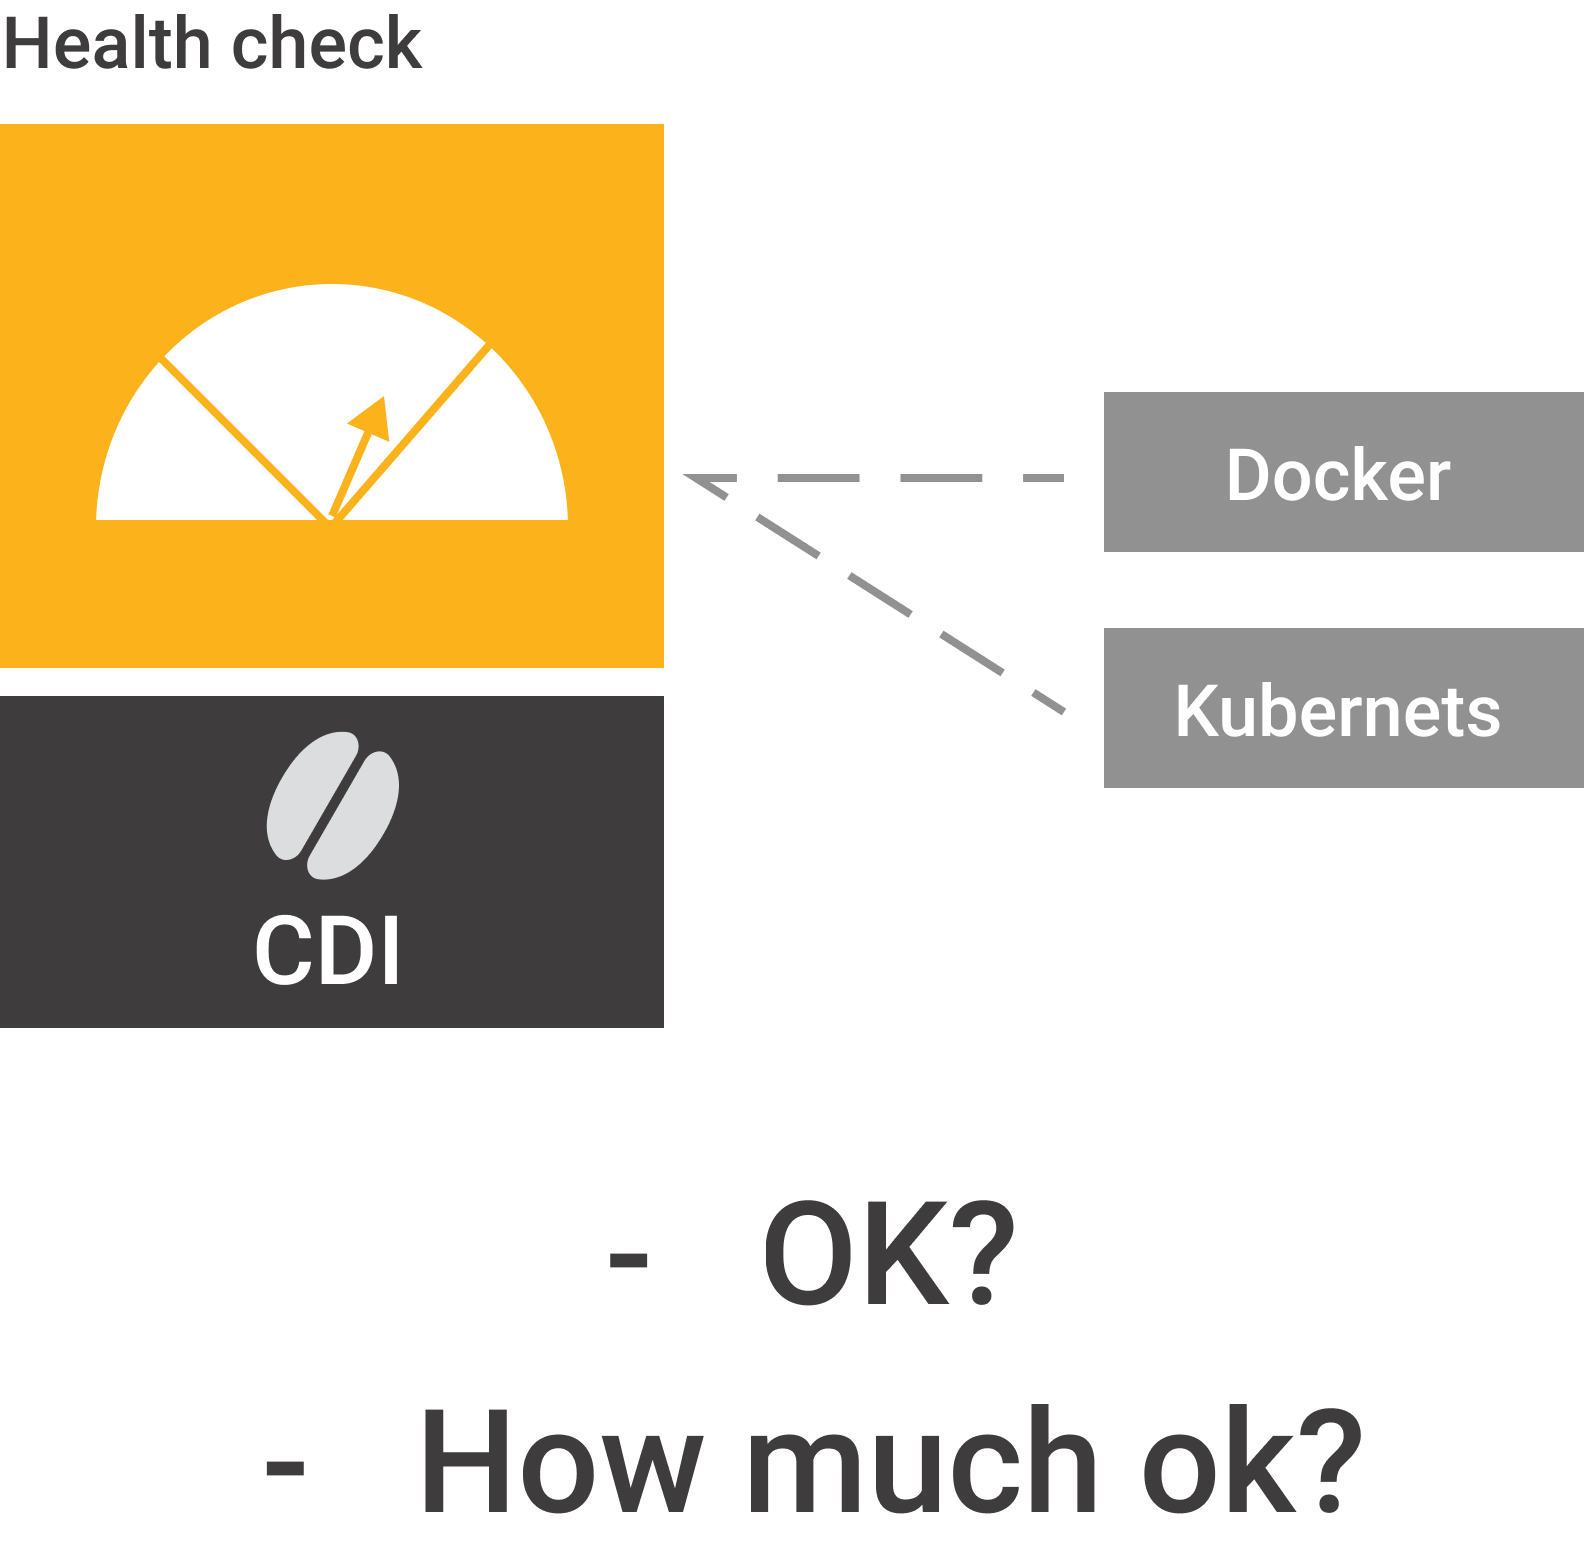
\includegraphics[width=0.75\linewidth]{Images/healthcheck}
\end{figure}
\end{frame}

\begin{frame}[fragile]{Health Check}
¿Estas vivo?
\begin{lstlisting}
@Override
public HealthCheckResponse call() {
	return HealthCheckResponse.named("TaVivoAinda")
		.withData("key1", "val1")
		.withData("key2", "val2")
		.up()
		.build();

}
\end{lstlisting}

\end{frame}


\begin{frame}{JWT}
\begin{figure}
	\centering
	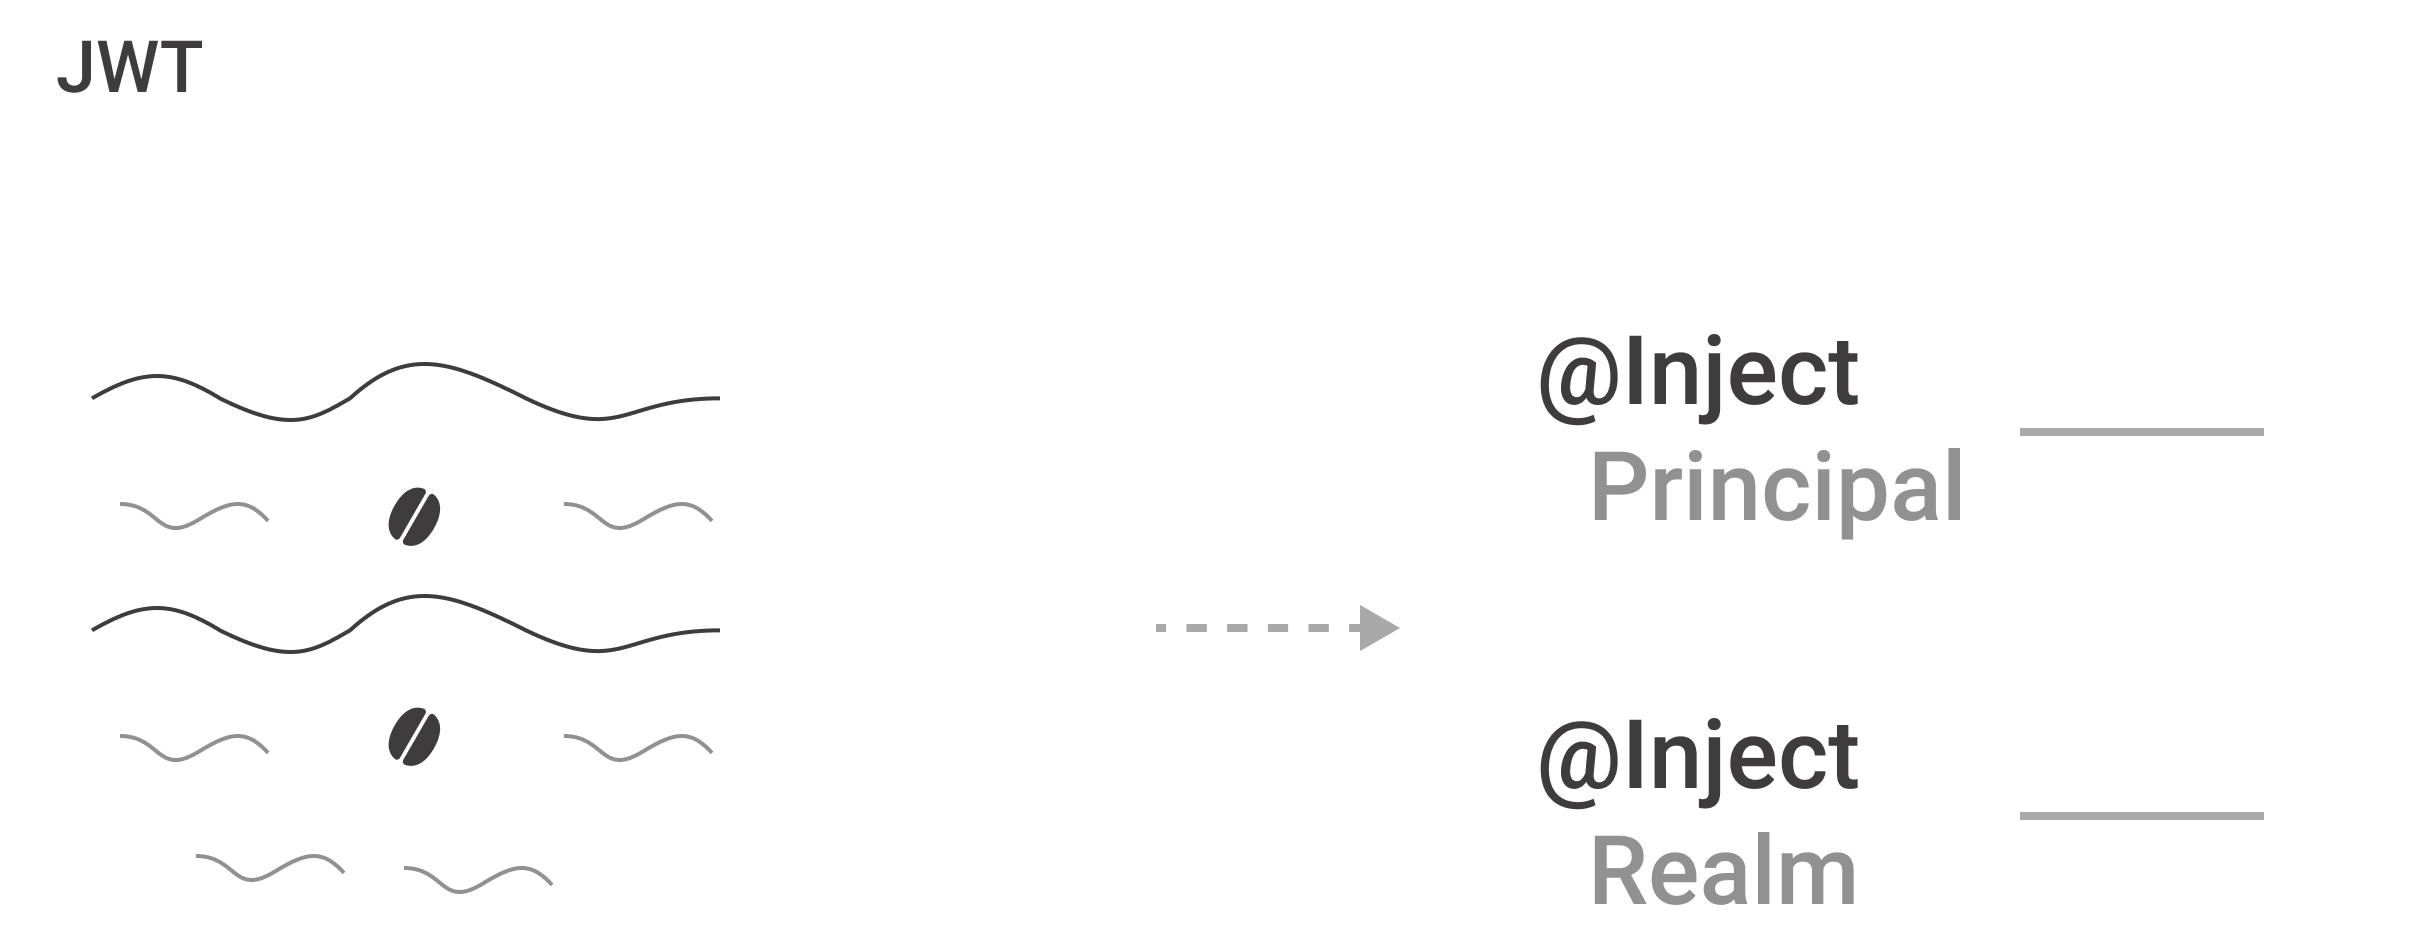
\includegraphics[width=0.9\linewidth]{Images/jwt}
\end{figure}
\end{frame}


\begin{frame}[fragile]{JWT}

\begin{lstlisting}
<@\textcolor{red}{@LoginConfig(authMethod = "MP-JWT")}@>
public class ApplicationConfig extends Application {
}
\end{lstlisting}

\begin{lstlisting}
@Inject
private JsonWebToken jwtPrincipal;

@Inject
<@\textcolor{red}{@Claim("email")}@>
private String email;
\end{lstlisting}
\end{frame}

\begin{frame}{TypeSafe}
\begin{figure}
	\centering
	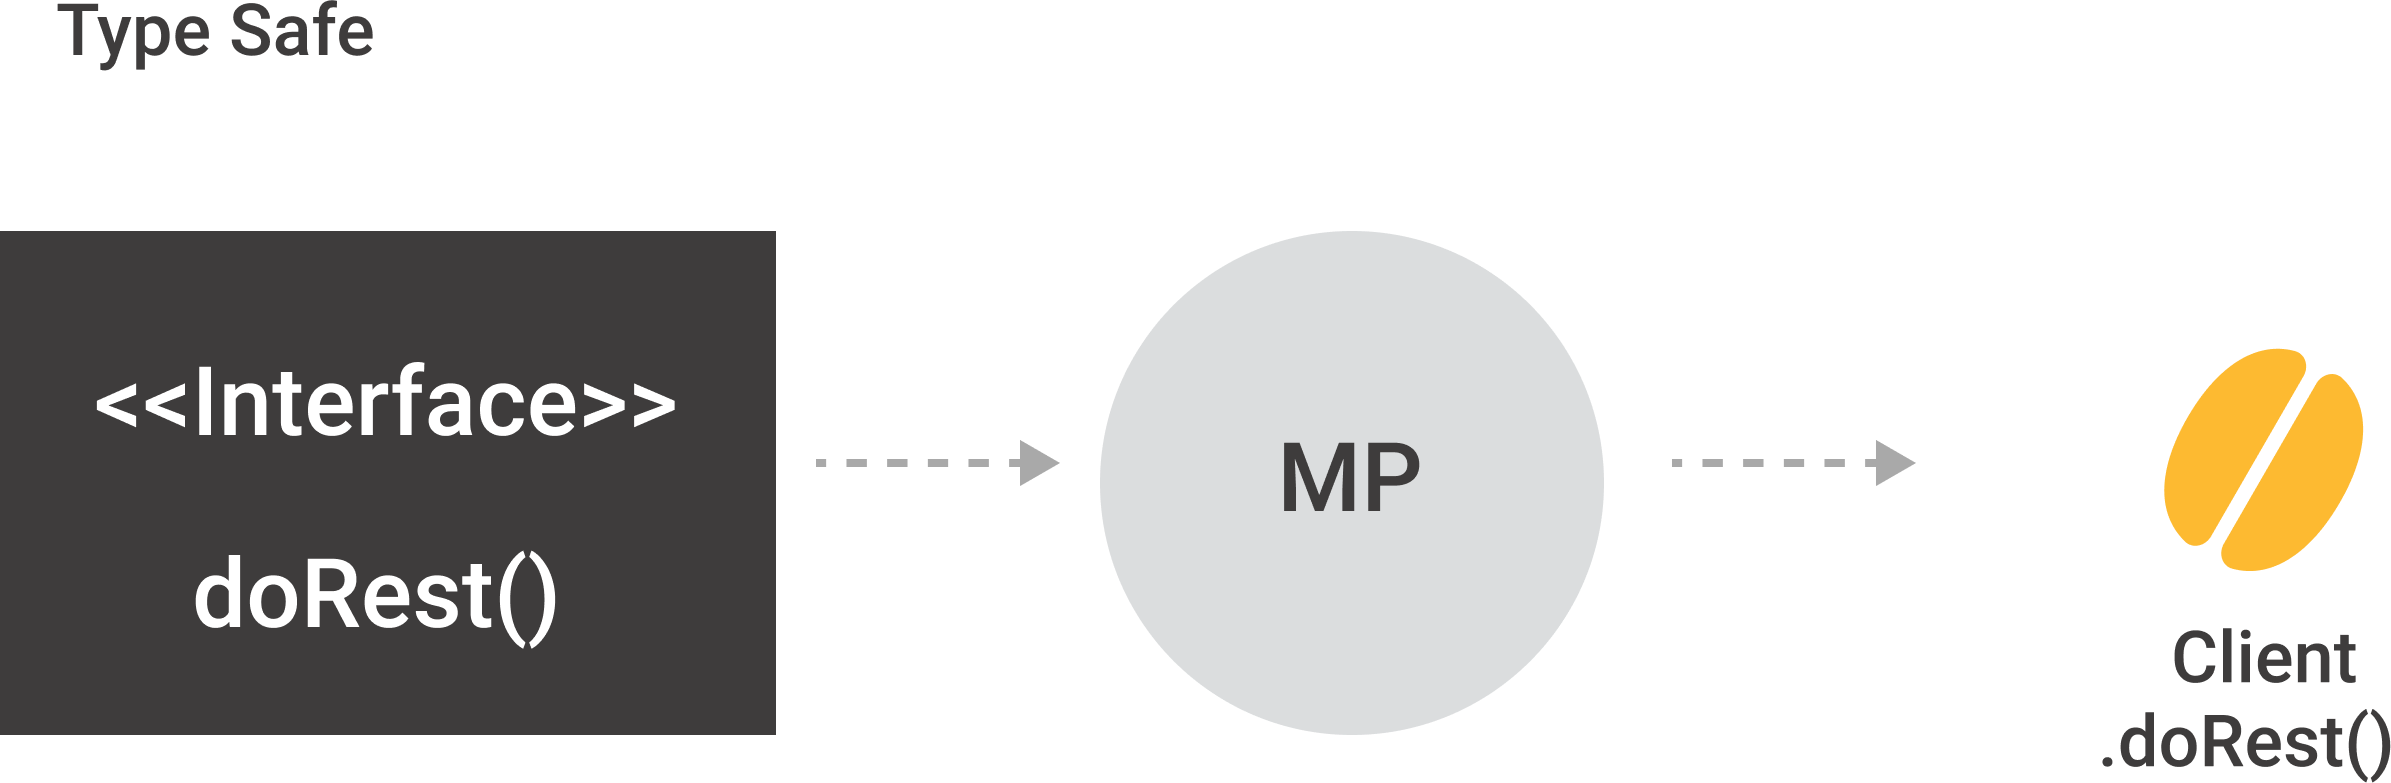
\includegraphics[width=0.75\linewidth]{Images/typesafe}
\end{figure}
\end{frame}

\begin{frame}[fragile]{TypeSafe}


\begin{lstlisting}
@Path("/playlist")
@Consumes("application/json")
public <@\textcolor{red}{interface}@> MusicPlaylistService {

	@GET
	List<String> getPlaylistNames();

	
	@PUT
	@Path("/{playlistName}")
	long updatePlayList(@PathParam("playlistName")
		String name,
		List<Song> playlist)
		throws UnknownPlaylistException;
}
\end{lstlisting}
\end{frame}





\begin{frame}{Víctor Orozco}
\begin{columns}[T] % contents are top vertically aligned
	
	\begin{column}[T]{4cm} % alternative top-align that's better for graphics
		\begin{figure}
			\centering
			
\includegraphics[width=\linewidth]{Images/logos}
		\end{figure}
	\end{column}
	\begin{column}[T]{6cm} % each column can also be its own environment
		\begin{itemize}
			\item vorozco@nabenik.com
			\item \href{https://twitter.com/tuxtor}{@tuxtor}
			\item \href{http://www.nabenik.com}{http://www.nabenik.com}
		\end{itemize}
	\begin{center}
		
\includegraphics[width=0.1\linewidth]{Images/cclogo}
		\\
		This work is licensed under a Creative Commons Attribution-ShareAlike 3.0.
	\end{center}
	\end{column}
\end{columns}
\end{frame}


\end{document}

s